
\section{Selection and Categorisation}\label{sec-selectionandcat}
Data collected by the ATLAS reconstruction consists of different types of low-level information measured in various sub-detectors. Different processing steps, collectively referred to as \textit{reconstruction}, must be applied to unlock a higher-level physical interpretation of the information: constructing tracks from hit in the silicon detectors, identifying electrons and muons, etc. This section introduces the object selection, listing the recipes applied to identify the different relevant physics objects. The analysis event selection, requiring different reconstructed objects to be identified in data and simulations, is then presented as well as the final categorisation separating events into defined analysis regions.

\subsection{Object Selection}\label{sec-obj}% TODO when writing the object part of detector, might have to simplify stuff % TODO should I mention truth tagging?
As introduced in Chapter \ref{chapter-ATLAS}, the ATLAS software supports different object reconstruction techniques. The reconstruction strategy of the relevant objects to the \vhbc\ analysis is presented in this section. 

\paragraph{Primary Vertex:} all events considered in the analysis are required to have at least one primary vertex reconstructed from tracks in the \gls{id} \cite{ATL-PHYS-PUB-2015-026}.

\paragraph{Electrons:} are reconstructed by matching a deposit in the electromagnetic calorimeter with a track in the \gls{id} \cite{Aaboud:2657964, Aad_2019}. Electrons are required to have $p_T > 7$ GeV and $|\eta|<2.47$. They are identified with a \textit{loose} working point of a likelihood discriminant, matching the calorimeter shower shape to an associated track. The $e$ candidates must satisfy $p_T$-dependent isolation criteria in both the \gls{id} and calorimeter. In the 1L channel, the \textit{tight} likelihood criterion is used with stricter calorimeter isolation requirements to better reject the multi-jet background. Additional requirements on the electron selection are lepton channel-dependent and summarised in Table~\ref{tbl:elOb}. $VH$-Loose electrons require a loose likelihood identification and are applied in all channels. Additionally, the $WH$-Signal and $ZH$-Signal criteria are respectively applied in the 1L and 2L channels, with a tighter $p_T$ due to the trigger threshold. The 1L likelihood identification and isolation selections are tighter to suppress the multi-jet background. % TODO reference the electron segment earlier in the thesis. % TODO Isolation should be define

\begin{table}[!htbp]
  \begin{center}
    %\resizebox{0.99\textwidth}{!}{
      \begin{tabular}{ccccccc} \hline \hline
        Selection & $p_T$ & $\eta$ & ID & $d_{0}^{\mathrm sig}$ w.r.t. BL &  $|\Delta{z_{0}}\sin\theta|$ & Isolation \\ \hline
        $VH$-Loose & $>$7 GeV & $|\eta|< 2.47$ & \textit{Loose} & $ <5$ & $<0.5$ mm & Loose \\ % Loose\_VarRad
        $ZH$-Signal & $>$27 GeV & $|\eta|< 2.47$ & \multicolumn{3}{c}{Same as $VH$-Loose} \\
        $WH$-Signal & \multicolumn{2}{c}{Same as $ZH$-Signal} & \textit{Tight} & \multicolumn{2}{c}{Same as $ZH$-Signal} & Strict \\ %HighPtCaloOnly
        \hline\hline
      \end{tabular}
    %}
    \caption{Electron Selection requirements.} % TODO Define BL and d0
    \label{tbl:elOb}
  \end{center}
\end{table}

\paragraph{Muons:} are reconstructed by matching an energy deposit in the muon detector with information from the \gls{id} and \glsfirst{ms} \cite{Aad:2746302}. They are required to have $p_T >$ 7 GeV, $|\eta| < 2.7$, to satisfy a \textit{loose} identification criteria, and be isolated in the \gls{id} according to $p_T$-dependant criteria. These requirements are summarised in Table~\ref{tbl:muonOb} and vary depending on the lepton channel similarly to the electron requirements. The $VH$-Loose requirements are applied to muons in all channels. The $WH$-Signal and $ZH$-Signal are additionally applied to the 1L and 2L channels respectively, with a stricter track-based isolation used in 1L to suppress the multi-jet background.

\begin{table}[!htbp]
    \begin{center}
      \resizebox{\textwidth}{!}{
        \begin{tabular}{ccccccc} \hline \hline
          Selection & $p_T$ & $\eta$ & ID & $d_{0}^{\mathrm sig}$ w.r.t. BL  & $|\Delta{z_{0}}\sin\theta|$ & Isolation \\ \hline
          $VH$-Loose & $>$7 GeV & $|\eta|< 2.7$ & Loose & $ <3$ & $<0.5$ mm & Loose \\ % Loose\_VarRad
          $ZH$-Signal & $>$27 GeV & $|\eta| < 2.5$ & \multicolumn{4}{c}{Same as $VH$-Loose} \\
          %WH-Signal & $>$25 GeV ($>$27 when $p_T^V<$ 150 GeV) & $|\eta|< 2.5$ & Medium quality & $ <3$ & $<0.5$ mm & HighPtTrackOnly \\
          $WH$-Signal & \makecell[c]{$>$25 GeV if $p_T^V>$ 150 GeV\\ $>$27 GeV if $p_T^V<$ 150 GeV} & $|\eta|< 2.5$ & Medium & $ <3$ & $<0.5$ mm & Strict \\
          \hline\hline
        \end{tabular}
      }
      \caption{Muon Selection requirements.} % TODO Define BL and d0
      \label{tbl:muonOb}
    \end{center}
  \end{table}
  
\paragraph{Taus:} hadronically decaying $\tau$-leptons are identified and vetoed in 1L using an \gls{rnn}-based tagger \cite{ATL-PHYS-PUB-2019-033}. Taus are required to have a $p_T >$ 20 GeV, $|\eta| <$ 2.5, and to have 1 or 3 associated tracks. In 0L and 2L, if the jet passes a \textit{loose} working point requirement for hadronically decaying $\tau$-leptons, it is no longer considered a jet and cannot be considered as a candidate for the reconstruction of the Higgs boson. % TODO find more info from the object notes. % TODO also clarify this last thing about inclusive of tau events.

\paragraph{Missing Transverse Energy:} neutrinos are not detectable in ATLAS and their presence is inferred from momentum imbalance in the transverse plane to the beam axis. $E_T^{\textrm{miss}}$, also called MET, is the negative vectorial sum of the transverse momentum of physics objects, namely electrons, muons, hadronic $\tau$, and jets. An additional track-based \textit{soft term} is added, to include a contribution from good quality tracks associated with the \glsfirst{pv} but not to any reconstructed physics object \cite{ATLASmetReco}. % TODO This citation is from the VHcc, check in object note it's still relevant.

\paragraph{Jets} Three types of jets are used by the analysis, all reconstructed with the anti-$k_t$ algorithm \cite{Cacciari:2008gp}:
\begin{enumerate}
  \item Small-$R$ jets: are reconstructed from topological clusters of energy deposit in the hadronic calorimeter based on the reconstructed PFlow objects with a radius $R = 0.4$. A jet is considered as \textit{central} if $|\eta| < 2.5$ and $p_T$ > 20 GeV, and as \textit{forward} if 2.5 $\leq |\eta|$ < 4.5 and $p_T > 30$ GeV. Central (forward) jets with a $p_T < 60$ GeV ($p_T < 120$ GeV) are required to originate for the primary vertex as identified by the jet vertex tagger (\gls{jvt}) to limit the pile-up background \cite{atlasPUJVT}. \textit{Tight} jet cleaning criteria are applied to suppress non-collision background. Central jets are used in the resolved regime to reconstruct the Higgs candidate, based on flavour tagging. % TODO more detail on jet cleaning criteria.
  \item Large-$R$ jets: are similar to small-$R$ jets with a larger radius $R = 1.0$, and required to have $p_T > 250$ GeV and $|\eta| < 2$. They are used in the boosted regime to reconstruct the Higgs candidate. 
  \item Variable-$R$ (\gls{vr}) track-jets: are reconstructed with a $p_T$-dependent radius, optimised for double $b$-tagging efficiency of the boosted $H \rightarrow b\bar{b}$ decays \cite{ATL-PHYS-PUB-2017-010}. They are required to have $p_T > 10$ GeV and $|\eta| < 2.5$. These track-jets are used to reconstruct the $b$-tagged objects inside the large-$R$ jet and to define a boosted control region rich in the top background. 
\end{enumerate}
%TODO missing all of the corrections 

\paragraph{Flavour Tagging:} Jet flavour tagging is perhaps the most important part of the event reconstruction. The latest available \gls{dl1r} tagger from Run 2 is used in the analysis for both $b$- and $c$-tagging in the resolved and boosted regime \cite{atlas:FTAGRUN2}. The methodology differs slightly between the two regimes of the analysis due to the different flavour tagging needs:  % TODO the calibration must be more detailed
\begin{itemize}
  \item In the resolved \vhbc, \gls{dl1r} is used to tag both $b$- and $c$-jets. The so-called \glsfirst{pcft} scheme, illustrated in Figure~\ref{fig:pseudotag}, is deployed to allow for a coherent joint definition and simultaneous calibration of $b$- and $c$-tagged jets, adopting the technique first introduced for 2D $c$-tagging in the \vhc\ analysis \cite{Collaboration:2721696}. The \gls{dl1r} tagger assigns a $b$-score\footnote{With an $f_c = 0.018$ value.} and a $c$-score\footnote{With an $f_b = 0.3$ value.} to every selected jets. To tag a jet, the associated score must be higher than a specific cutoff value, defined to give a specific selection efficiency in simulated data, also known as a \glsfirst{wp}. From this score, the jet is assigned one of 4 possible labels, based on 2 $b$-tagging \gls{wp} and 2 $c$-tagging \gls{wp}. These \gls{wp} are tested in strict successive order, with first a 60\% tight $b$-tagging working point (bin 4) followed by a looser 70\% $b$-\gls{wp} (bin 3). A jet passing these selections is labelled $B$\footnote{The difference between these $b$-tagged is used in the discriminant \gls{mva} of the analysis}. Otherwise, it is considered for $c$-tagging with first a \textit{tight} working point at 20\% efficiency (bin 2), followed by a \textit{loose} \gls{wp} at an exclusive efficiency of 20\% (bin 1) on the remaining jets - so that 40\% of the $c$-jets are effectively selected in the combined tight and loose bins. A jet selected by the tight $c$-tagging \gls{wp} is labelled $T$, and $L$ if it only passes the loose \gls{wp}. A jet failing to pass all \glspl{wp} is not tagged and labelled $N$ (bin 0). The $b$-tagging \glspl{wp} correspond to official ATLAS ones for \gls{dl1r} \cite{atlas:FTAGRUN2}, while those for $c$-tagging are optimised for the purpose of the analysis. The tagging efficiency of each bin is displayed in Table~\ref{tbl:PCFTtageff}, shown for the main flavours as well as $\tau$-leptons reconstructed as jets.
  \begin{table}[h!]
    \begin{center}
        \begin{tabular}{c|c|cccc}
          \hline \hline
          \multirow{2}{*}{PCFT bin} & \multirow{2}{*}{PCFT bin name} & \multicolumn{4}{c}{Jet tagging efficiency $\epsilon_{jet}$}\\
          & & $b$-jet &  $c$-jet &  light-jet & $\tau$-jet \\ 
          \hline
          1 & $c$-loose & 11.5\% & 20.5\% & 6.5\%   & 18.5\%\\
          2 & $c$-tight & 4.8\%  & 24.2\% & 0.9\%   & 19.5\%\\
          3 & $b$-70\%  & 11.2\% &  5.2\% & 0.13\%  &  1.7\%\\
          4 & $b$-60\%  & 58\%   & 2.65\% & 0.051\% & 0.49\%\\
          \hline \hline
        \end{tabular}
      \caption{Jet tagging efficiency for $b$-jet, $c$-jet, light-jet and $\tau$-jet in the \glsfirst{pcft} bins, measured from a \textsc{Powheg}+\textsc{Pythia} 8 simulated sample of semi-leptonic \ttb\ events.}
     \label{tbl:PCFTtageff} % Don't understand why thigh is not at 20\%
    \end{center}
  \end{table}
  The calibration of all five bins of Figure~\ref{fig:pseudotag} is performed simultaneously for the analysis following the methodology described in Ref \cite{atlas:FTAGRUN2}, with some results presented in Appendix \ref{appsec-vh-ftagcal}.
  \begin{figure}[h!]
    \center
      \begin{minipage}[c]{0.69\textwidth}
        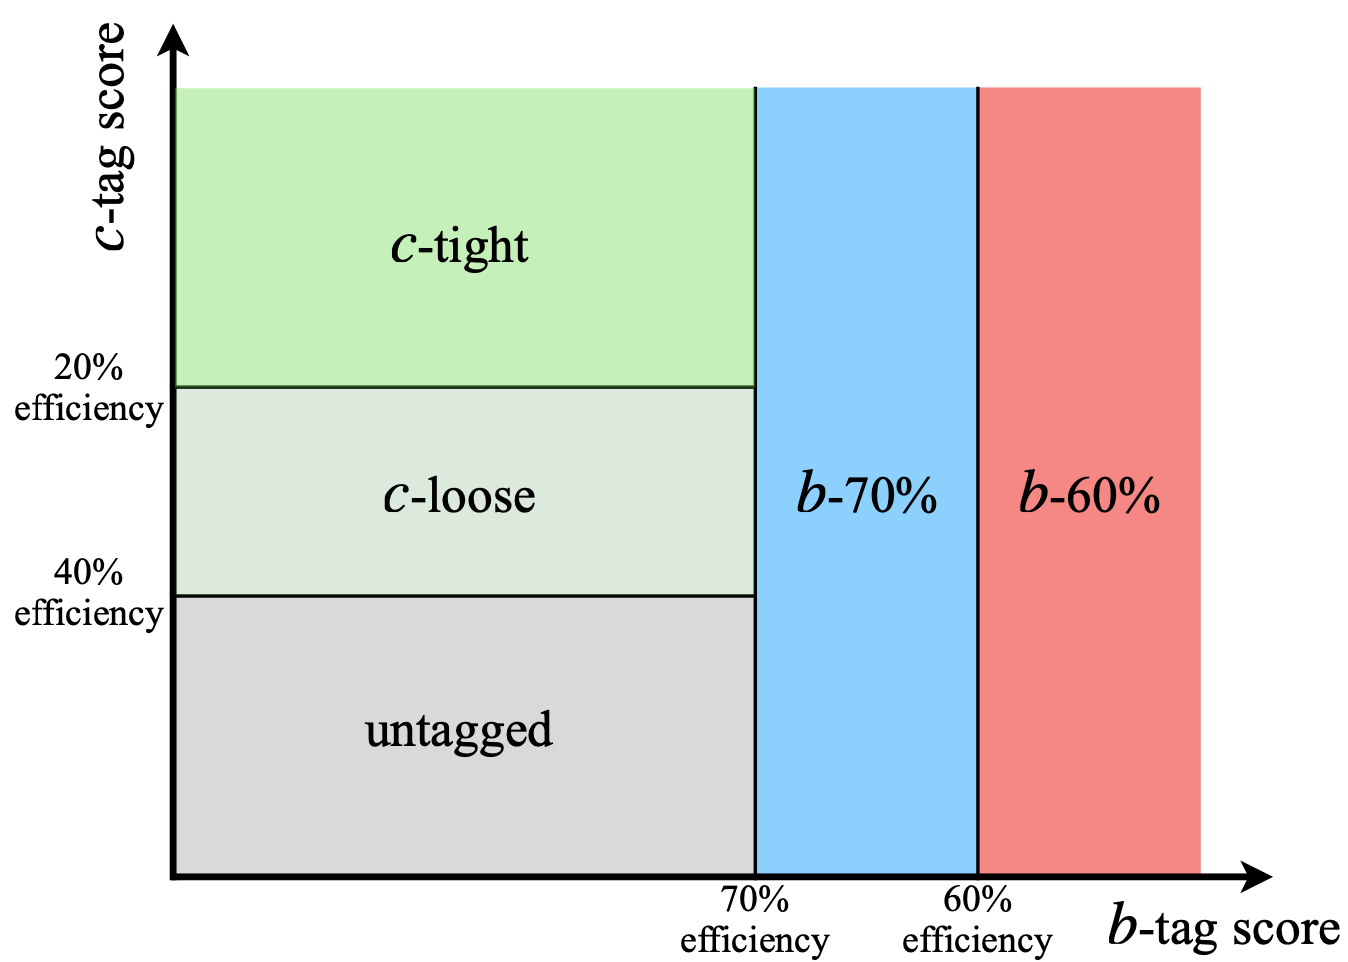
\includegraphics[width=0.98\textwidth]{Images/VH/pseudocontinuous.png}
      \end{minipage}
      \begin{minipage}[c]{0.3\textwidth}
        \caption{The \glsfirst{pcft} scheme used to simultaneously define 2 $b$-tagged, a tight $c$-tagged, a loose $c$-tagged, and a non-tagged bins.} 
        \label{fig:pseudotag}
      \end{minipage}
  \end{figure}

  \item The boosted regime only targets $b$-jets, with the single-jet \gls{dl1r} tagger used. As such, the standard pseudo-continuous $b$-tagging method is used \cite{atlas:FTAGRUN2}. The track-jets associated with the leading large-$R$ jet are given a $b$-score based on the per-flavour probabilities outputted by \gls{dl1r}. The 85\% working point is adopted to maximise the signal yield, due to the important statistical limitations in the boosted regime. Track-jets passing this working point are $B$-tagged, otherwise, they are untagged $N$. Studies showed that the very loose \gls{dl1r} \gls{wp} gives a better expected statistical significance than the then-available $X_{bb}$ tagger. The official calibration from Ref \cite{atlas:FTAGRUN2} is used and extended to higher $p_T$ with uncertainty extrapolation due to the wide range of $p_T$ probed in the analysis, as presented in Appendix \ref{appsec-vh-ftagcal}.
\end{itemize}
While the analysis was underway, the superior single-jet \gls{gnn} taggers and the boosted objects $GN2X$ tagger introduced in Chapter \ref{chap-ftag} were not yet available as their calibration was an ongoing effort. Furthermore, switching to these new taggers was not feasible from a practical point of view in the timing of the analysis. They represent, however, an exciting avenue for progress in future iterations of this search, in both the resolved and boosted regimes. \\ % TODO check how the wp are defined %TODO also check the fc alue

\paragraph{Object Overlap:} overlap removal is applied to avoid double-counting electrons, muons, small-$R$ and large-$R$ jets, and hadronically decaying $\tau$-leptons passing the object selection.

\subsection{Event Selection}\label{sec-regimeCat}
A subset of all the events recorded by ATLAS during Run 2 is selected for further selection based on specific triggers. The trigger selections of the \vhb\ and \vhc\ have been harmonised for the combined analysis, and are specified per lepton channel in 0-lepton (0L), 1-lepton (1L), and 2-lepton (2L). In 0L, events are selected using the lowest un-prescaled \etm\ trigger, with an increasing lower threshold rising from 70 GeV for data recorded in 2015, 90 to 110 GeV for 2016, and to 110 GeV for 2017 and 2018 due to higher trigger rate later in Run 3. The 1L channel triggers cover both the $e$ and the $\mu$ sub-channels. For the $e$-channel, single electron events must be triggered by the lowest un-prescaled single electron trigger. For muons, the \etm\ trigger of 0L is used for events with \ptv\ > 150 GeV, while the lowest un-prescaled single muon trigger is used for events with a lower \ptv. Finally, the triggers for 2L are equivalent to 1L except for the muon channel where the \ptv\ threshold for switching between triggers is raised to 250 GeV. The use of \etm\ trigger at high \ptv\ for muons was shown to increase the signal acceptance by $\sim$ 5\%.\\ % TODO missing boosted no? % Hidding this trigger thingFurther details on the trigger setup are given in Table~\ref{aptab:trigs2015_to_2018} of the Appendix.


The different regimes of the analysis are defined by flavour tagging and the strategy to reconstruct the Higgs boson. In the resolved regime, an event must have at least two central jets. Two candidate jets are selected to reconstruct the Higgs using the so-called \textit{All Signal Jets} strategy and define an event tag by combining their individual tags. A hierarchy of tags is introduced, following the ordering: $B$ > $T$ > $L$ > $N$. The pair of candidates is selected from the two central jets having the highest tags, and the highest $p_T$ in case of ties. Events are labelled based on the tag of the selected jets, e.g., $TT$ is assigned to events with 2 tight $c$-tagged jets and no $b$-jet and $BL$ to events with a $b$-tagged and a loose $c$-tagged jets. In the boosted regime, at least 2 track-jets are required to be associated with the large-$R$ jet leading by $p_T$, and the tags of the 3 track-jets with the highest $p_T$ are considered for the event. This labelling and the reconstructed \ptv\ define the different regimes of the resolved and boosted \vhb\ and \vhc\ parts of the combined analysis. To fully reconstruct the Higgs boson from the two candidate jets or the large-$R$ jet, additional selections are applied.

\paragraph{Higgs candidates in resolved regime:} for \vhb, the two candidates must be $b$-tagged (bins 3 and 4) with no additional $B$- and tight $c$-tagged jets allowed\footnote{In 2L, additional $T$-tagged jets are allowed due to the limited statistics and the different derivation of the top \gls{cr} in 2L, requiring mixed leptons $e\mu$.}, while in \vhc\ no $b$-tagged jet is allowed and at least one of the candidates must be tight $c$-tagged ($T$). As described in the next section, two control regions are defined by changing this flavour selection: a Top \gls{cr}, combining at least 1 $B$-tag with at least 1 $T$-tag, and the $V+l$ requiring 1 loose $c$-tagged jet ($L$) with an untagged $N$ jet for \vhc. The Higgs candidates are sorted by $p_T$ into a leading $j_1$ and sub-leading $j_2$ candidates. The leading candidate must have $p_T > 45$ GeV, while other jets are required to have $p_T > 20 GeV$. The invariant mass of the Higgs candidate as measured by $m_{bb}$ ($m_{cc}$) must be above 50 GeV before applying energy corrections, to avoid the $V$+jets gluon splitting mis-modelling at low masses.  % TODO bc overlap in 2L VHbb: tight c jets are allowed? % TODO check V+l has LL LN, ... 
\paragraph{Higgs candidates in boosted regime:} the selection requires exactly 2 $B$-tags among the 3 track-jets leading by $p_T$ associated to the leading large-$R$ jet. The reconstructed mass of the Higgs candidate based on the leading-$R$ jet mass $m_J$ must satisfy $m_J > 50$ GeV, with a leading large-$R$ jet $p_T > 250$ GeV. \\

In all regimes, the number of reconstructed charged lepton in the final state defines three channels as the 0-lepton (0L), 1-lepton (1L), and 2-lepton (2L). The objective of this leptonic selection is to reconstruct the associated $V$-boson. The selection of events in the resolved regime is presented in Table~\ref{tbl:VHbbccevSelTable} and Table~\ref{tbl:VHbbBoostevSelTable} for the boosted regime. Additional channel-specific requirements are also introduced to limit background contamination and reviewed in this section.

\subsubsection{Selection specific to the 0-lepton channel}\label{subsubsec-0Lsel}
In the 0-lepton channel, 0 $VH$-loose leptons should be selected and \etm\ should be $>$ 150 GeV ($>$ 250 GeV) in the resolved (boosted) regime, to identify the decay $Z \rightarrow \nu\nu$. \\ % TODO Conflict in the main note: selection is 200 in text for boosted and 250 in the table.
 
In the resolved regime, the scalar sum $S_T$ of the jet $p_T$ in the events must be $> 120$ GeV ($> 150$ GeV) for 2-jets ($\geq$ 3 jets) to avoid a mis-modelled region in simulation due to the triggers. In the case of a decaying $W \rightarrow \tau \nu$ followed by a hadronic decay of the $\tau$-lepton which is reconstructed as a jet, there are no electrons nor muons in the final state. To limit this $\tau$-contamination in the 0L channel, an extra selection is applied when at least 1 hadronic $\tau$ is reconstructed: the reconstructed transverse $W$ mass \[ m_T^W = \sqrt{2 p_T^l E_T^{\textrm{miss}} (1 - \cos(\Delta \phi(l, E_T^{\textrm{miss}} ) ) ) } \] is required to be $m_T^W \geq$ 10 GeV, with the $W$-boson $p_T$ estimated from the vectorial sum of the leading hadronic $\tau$ momentum ($p_T^l$) and \etm\ instead of \ptv.\\

To limit the multi-jet background, so-called \textit{anti-QCD cuts} using the azimuthal angle $\phi$ are applied in all regimes:
\begin{itemize} % TODO what is this azimuthal angle
    \item For resolved only, $|\Delta \phi(j_1, j_2)| < 140 \ensuremath{^\circ}$.
    \item $|\Delta \phi(E_t^{\textrm{miss}}, H)| > 120 \ensuremath{^\circ}$.
    \item $\textrm{min}|\Delta \phi (E_T^{\textrm{miss}}, \textrm{ jet})|$ must be $> 20\ensuremath{^\circ}$ ($> 30 \ensuremath{^\circ}$) for resolved 2-jet (3-jet) events and $> 30\ensuremath{^\circ}$ for the boosted regime.
\end{itemize}
The cuts are tuned to limit the multi-jet contamination to a fraction of order 1\% of the total background in 0L, making the multi-jet negligible in the 0-lepton channel. 

\subsubsection{Selection specific to the 1-lepton channel}
In the 1L channel, the targeted decaying vector boson is a $W \rightarrow \ell\nu$, with $\ell = e, \mu$. Exactly 1 $WH$-signal lepton is required, with events having more than 1 $VH$-loose lepton vetoed\footnote{The $VH$-loose lepton is at best the $WH$-signal lepton.}. The vector boson is reconstructed from the vectorial sum of the \etm\ and the lepton transverse momentum identified in the event, with a \ptv\ $> 75$ GeV. To suppress the multi-jet background, events with one electron are required to have an \etm\ $>$ 30 GeV ($> 50$ GeV) in the resolved (boosted) regime, with a reconstructed $m_T^W > 20$ GeV for events with low $W$ transverse momentum $p_T^V < 150$ GeV. For the resolved $\mu$-channel, as the same \etm\ trigger is used as in the 0L, the scalar sum of $p_T$ is similarly restrained with $S_T > 120$ GeV ($> 150$ GeV) for 2-jets ($\geq$ 3 jets). A significant background in the 1-lepton channel is the \ttb, with both $t$-quarks decaying into a $W$ boson and a $b$-quark. Events where one of the $W$ boson decay follows $W \rightarrow \tau \nu$ with the $\tau$ decaying hadronically and the other $W$ decays into an $e$ or a $\mu$ have the same leptonic signature as the signal. A strict hadronic $\tau$-veto is applied in all regimes to suppress this background. Events passing the 0-lepton selection with $\geq 1$ hadronic taus are moved to the 1-lepton channel with the leading hadronic $\tau$ used to reconstruct variables requiring an $e$ or a $\mu$. This migration is performed to recover the estimated $~10$\% ($\sim$ 20\%) of $WH$ signal where $W\rightarrow \tau \nu$ with a hadronically decaying $\tau$-lepton in the resolved (boosted) regime, and help decorrelate the $WH$ and $ZH$ measurements in the \vhb\ side.

\subsubsection{Selection specific to the 2-lepton channel}
The 2L channel targets the associated bosonic decay where $Z \rightarrow\ell\ell$, with the $Z$ reconstructed from two $VH$-loose leptons required to have the same flavour, with at least one passing the $ZH$-signal lepton requirements. In the di-muon channel, the leptons are further required to be of opposite charges\footnote{This is not applied to the di-electron channel due to a significantly higher charge mis-identification.}. The invariant mass of the di-lepton system is required to be consistent with the $Z$ mass with $81 < m_{ll} < 101$ GeV in the resolved and $66 < m_{ll} < 111$ GeV in the boosted regime, to suppress non-resonant lepton-pair producing background such a \ttb\ and multi-jet. The leptons must satisfy $p_T > 25$ GeV, with a stricter $p_T > 27$ GeV required for the leading muon when the event is selected by the muon trigger.

\begin{table}[htbp] % TODO maybe vertical alignment?
  \resizebox{1\textwidth}{!}
  {
  \renewcommand*{\arraystretch}{1.1}
  \begin{tabular}{C{3.3cm}|C{2.8cm}|C{2.5cm}|C{1.8cm}|C{2.5cm}|C{1.8cm}}
  \hline \hline
  Selection & 0-Lepton & \multicolumn{2}{c|}{1-Lepton} & \multicolumn{2}{c}{2-Lepton}  \\
  & & $e$-channel & $\mu$-channel & $e$-channel & $\mu$-channel \\ \hline \hline
  Trigger & \etm\ & Single electron & \etm\ & Single electron & \etm\ \\
  Leptons & 0 $VH$-loose lepton & \multicolumn{2}{c|}{1 $WH$-signal lepton} & \multicolumn{2}{c}{$\geq$ 1 $ZH$-signal lepton} \\
   & & \multicolumn{2}{c|}{No second $VH$-loose lepton} & \multicolumn{2}{c}{2 $VH$-loose leptons} \\
   &  & \multicolumn{2}{c|}{No hadronic $\tau$} & \multicolumn{2}{c}{Same flavour leptons} \\
   &  &  \multicolumn{2}{c|}{} & \multicolumn{2}{c}{Opposite charge for $\mu\mu$} \\ \hline
  \ptv\ &  \multicolumn{5}{c}{$>$ 400 GeV} \\
  Large-$R$ jet & \multicolumn{5}{c}{$\geq$ 1 large-$R$ jet ($R$ = 1.0), $p_T >$ 250 GeV, $|\eta| < 2$} \\
  Track-Jets & \multicolumn{5}{c}{$\geq$ 2 track-jets ($p_T > 10$ GeV, $|\eta| < 2.5$) matched to the leading large-$R$ jet} \\
  Tagging & \multicolumn{5}{c}{Exactly 2 of the 3 leading track-jets matched to the large-$R$ jet must be $b$-tagged} \\
  $m_J$ & \multicolumn{5}{c}{$> 50$ GeV} \\ \hline
  \etm\ & $>$ 200 GeV & $>$ 50 GeV & - & \multicolumn{2}{c}{-} \\ % TODO For 0L, it's 200 in the text but 250 in the table
  $|\Delta\phi(E_T^{\textrm{miss}}, H)|$ & $> 120\ensuremath{^\circ}$ & \multicolumn{2}{c|}{-} & \multicolumn{2}{c}{-} \\
  $\min |\Delta\phi(E_T^{\textrm{miss}}, \textrm{jets})|$ & $> 30\ensuremath{^\circ}$ & \multicolumn{2}{c|}{-} & \multicolumn{2}{c}{-} \\
  $m_{\ell\ell}$ & - & \multicolumn{2}{c|}{-} &  \multicolumn{2}{c}{$66$ GeV $< m_{\ell\ell} < 116 $ GeV} \\ \hline \hline
  \end{tabular}
  }
  \caption{Summary of the event selection in the 0-, 1- and 2-lepton channels of the boosted \vhb\ regime.} % TODO ADAPT THE LEGEND FOR WHAT IS PRESENTED
  \label{tbl:VHbbBoostevSelTable}
\end{table}

\clearpage

\begin{table}[h!]
    \begin{center}
    \resizebox{1\textwidth}{!}
    {

    \renewcommand*{\arraystretch}{1.1}
    \begin{tabular}{C{6cm}|C{4cm}|C{4cm}}
    \hline \hline
    Resolved Analysis Regime & $VH(H\rightarrow b\bar{b})$ & $VH(H\rightarrow c\bar{c})$ \\
    \hline \hline
    \multicolumn{1}{c}{}  &\multicolumn{2}{c}{Common Selections}\\ \hline 
    Jets & \multicolumn{2}{c}{$\geq$ 2 signal jets}  \\
    Candidate jets tagging &  2 $B$-tags & $\geq1$ $T$-tag, no $B$-tag \\
    Leading Higgs ($H$) candidate jet $p_T$ & \multicolumn{2}{c}{$>$ 45 GeV} \\
    Sub-leading $H$ candidate jet $p_T$ & \multicolumn{2}{c}{$>$ 20 GeV} \\
    $m_{bb}$ or $m_{cc}$ & \multicolumn{2}{c}{> 50 GeV (before correction)} \\ 
    Non-$H$ candidate jet $p_T$ & \multicolumn{2}{c}{$>$ 20 GeV ($> 30$ GeV for nJet categorisation only)} \\
    Candidate jets $\Delta R$  & \multicolumn{2}{c}{Upper cut $\Delta R \leq \pi$} \\

    \hline \hline 
    \multicolumn{1}{c}{} &\multicolumn{2}{c}{0-Lepton (0L)} \\
    \hline
    Trigger & \multicolumn{2}{c}{$E_T^{\textrm{miss}}$ triggers} \\
    Jets & $\leq$ 4 jets & $\leq$ 3 jets \\
    Additional jets tagging & no $T$-tag & no $B$-tag \\
    Top CR tagging & \multicolumn{2}{c}{$\geq$1 $B$-tag + 1 $T$-tag} \\
    Leptons & \multicolumn{2}{c}{0 $VH$-loose lepton} \\
    $E_T^{\textrm{miss}}$ & \multicolumn{2}{c}{$>$ 150~GeV}  \\
    $E_{T, trk}^{\textrm{miss}}$  & - & $>$ 30~GeV \\
    $S_T = \sum p_T^{\textrm{jets}}$ & \multicolumn{2}{c}{$>$ 120 GeV (2 jets), $>$150 GeV ($\geq3$ jets)}  \\ 
    $m_T^W$ & \multicolumn{2}{c}{$>$ 10 GeV when $\geq$ 1 hadronic $\tau$} \\
    $|\Delta\phi(j_1, j_2)|$ & \multicolumn{2}{c}{$< 140\ensuremath{^\circ}$} \\
    $|\Delta\phi(E_T^{\textrm{miss}}, H)|$ & \multicolumn{2}{c}{$> 120\ensuremath{^\circ}$} \\
    $\textrm{min}|\Delta \phi (E_T^{\textrm{miss}}, \textrm{jet})|$& \multicolumn{2}{c}{$>20\ensuremath{^\circ}$ (2 jets), $> 30\ensuremath{^\circ}$(3 jets)} \\

    \hline\hline 
    \multicolumn{1}{c}{} & \multicolumn{2}{c}{1-Lepton (1L)} \\
    \hline
    Trigger &  \multicolumn{2}{c}{$e$-channel: single electron trigger} \\
            & \multicolumn{2}{c}{$\mu$-channel: single muon trigger ($p_T^V <$ 150 GeV)} \\
            & \multicolumn{2}{c}{and 0L $E_T^{\textrm{miss}}$ triggers} \\
    Jets & \multicolumn{2}{c}{$\leq$ 3 jets}  \\
    Additional jets tagging & no $T$-tag & no $B$-tag \\
    Top CR tagging & \multicolumn{2}{c}{$\geq$1 $B$-tag + 1 $T$-tag} \\ % TODO fix the footnoteref
    hadronic $\tau$-veto & \multicolumn{2}{c}{no hadronic $\tau$} \\ 
    Leptons & \multicolumn{2}{c}{1 $WH$-signal lepton} \\
            &  \multicolumn{2}{c}{veto if $>1$~$VH$-loose lepton} \\
    $E_T^{\textrm{miss}}$   & \multicolumn{2}{c}{$>$ 30~GeV ($e$-channel)} \\
    $S_T$ & \multicolumn{2}{c}{Same as 0L for $\mu$ with \etm\ trigger}  \\ 
    $m_T^W$ & \multicolumn{2}{c}{$>$ 20 GeV for 75 < \ptv\ < 150 GeV} \\ 

    \hline\hline 
    \multicolumn{1}{c}{} & \multicolumn{2}{c}{2-Lepton (2L)}\\
    \hline
    Trigger &  \multicolumn{2}{c}{Same as 1L, \ptv\ $<$ 250 GeV for single $\mu$ trigger}\\
    Additional jets tagging & - & no $B$-tag \\
    Leptons & \multicolumn{2}{c}{2 $VH$-loose leptons} \\
            & \multicolumn{2}{c}{($\geq$ 1 $ZH$-signal lepton)} \\
            & \multicolumn{2}{c}{Same flavour, opposite-charge for $\mu\mu$} \\
    Top CR  & \multicolumn{2}{c}{Mixed $e\mu$ flavour} \\ 
    $m_{\ell\ell}$   & \multicolumn{2}{c}{81 $<$ $m_{\ell\ell}$ $<$ 101~GeV} \\
    \hline\hline
    \end{tabular}
    }
    \caption{Summary of the event selection in the 0-, 1- and 2-lepton channels of the resolved \vhbc\ regimes. The resolved 1L \& 2L Top CR tagging definition ignores the candidate jet tagging requirements For \vhc, an extra CR for \vlf\ changes the candidates tagging to one $L$-tag + no-tag ($LN$).} 
    \label{tbl:VHbbccevSelTable}
    \end{center}
\end{table}

\clearpage 
\subsection{Event Categorisation}\label{sec-eventCat}
Selected events are further categorised following a successive decomposition into regions of defined tag, vector boson $V$ transverse momentum $p_T^V$, and number of jets \nj. The full categorisation gives rise to signal and control regions that enter the statistical analysis defined in the fit framework of Section~\ref{sec-fitFramework}. The control regions are defined to help constrain the modelling of specific backgrounds, such as by correcting their yields. The definition of the regions depends on the analysis regime and the targeted Higgs decay, with Figure~\ref{fig:ana-strat-det} providing a condensed global overview of the different regions defined.

\subsubsection{Resolved Regime Categorisation}
In the resolved regime, the number of central + forward jets in an event defines different \nj\ categories, separated to maximise the signal sensitivity. A $p_T > 30$ GeV cut is considered for non-Higgs candidate jets just to determine this number of jets categorisation. This was found to limit the signal migration across \gls{stxs} bins in \vhb\ while having almost no impact on the \vhc\ sensitivity\footnote{It is nonetheless applied to harmonise the resolved regime.}. All distributions of the resolved regime regions with processes normalised to their posfit expectations from the fit described in Section~\ref{sec-fitFramework} are presented in Appendix \ref{appsec-vh-analRegResPosfit}. The plots presented in this section show the prefit and blinded distributions in the different regions, and simulated processes are therefore not normalised to data. The variables displayed correspond to those chosen for the fit, as detailed in Section~\ref{sec-vh-disc}. The precise definitions of the analysis regions are reviewed in this section.

\paragraph{Resolved \boldvhb\ SRs:} requires exactly 2 $b$-tagged jets ($BB$), with no extra $B$- nor any $T$-tags, and events are separated into different categories based on \nj. All lepton channels have a 2-jet and a 3-jet categories. The 0L channel has an additional 4-jet category, and the 2L an extra 4 or more jets (4p or $\geq$4) category\footnote{The 4/4p-jet category in 1L overlaps with the region used to calibrate the tagger and is rejected due to the \ttb\ limiting the sensitivity.}. They are included to improve the \gls{stxs} measurements sensitivity in bins with at least one additional jet. All regions are further split into different bins of $p_T^V$ as [75, 150] GeV (except for 0L\footnote{It is not feasible in 0L due to the trigger threshold on $E_T^{\textrm{miss}}$.}), [150, 250] GeV, and [250, 400] GeV. Selected \vhb\ signal regions in the analysis are presented in Figure~\ref{fig:plots_VHbb_ex_SR}. % TODO make sure that the ptv and nj are well alligned. It's more difficult as some nj are there only at some ptv.

\begin{figure}[h!]
  \centering
  \begin{subfigure}[b]{0.32\textwidth}
      \centering
      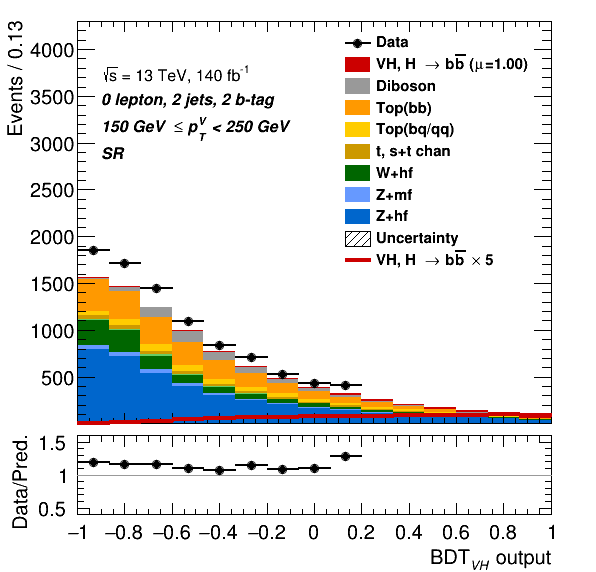
\includegraphics[width=\textwidth]{Images/VH/Own_fit/prefit_VHbb/Region_distmva_BMax250_BMin150_DSR_J2_TTypebb_T2_L0_Y6051_Prefit.png}
      \caption{0-lepton.}
      \label{fig:plots_VHbb_ex_OL_SR}
  \end{subfigure}
  \begin{subfigure}[b]{0.32\textwidth}
      \centering
      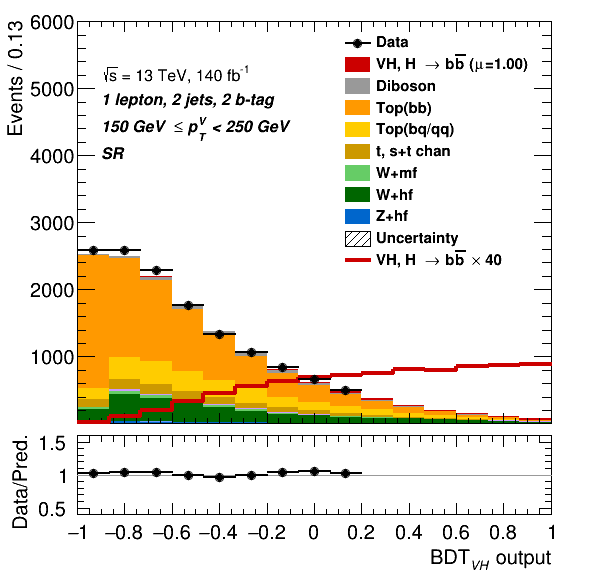
\includegraphics[width=\textwidth]{Images/VH/Own_fit/prefit_VHbb/Region_distmva_BMax250_BMin150_DSR_J2_TTypebb_T2_L1_Y6051_Prefit.png}
      \caption{1-lepton}
      \label{fig:plots_VHbb_ex_1L_SR}
  \end{subfigure}
  \begin{subfigure}[b]{0.32\textwidth}
    \centering
    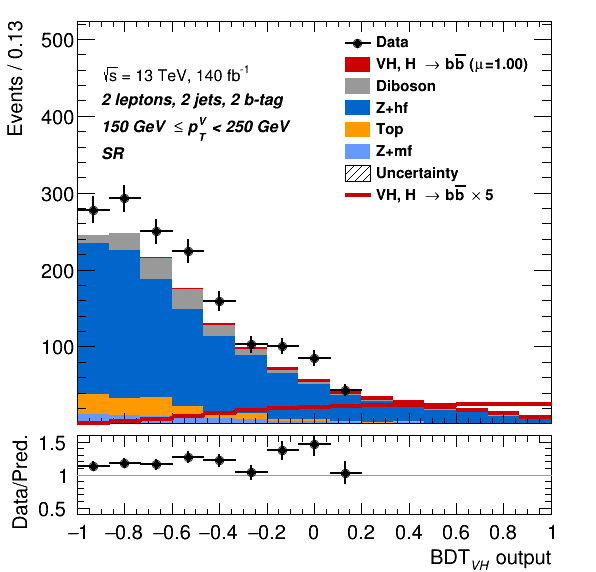
\includegraphics[width=\textwidth]{Images/VH/Own_fit/prefit_VHbb/Region_distmva_BMax250_BMin150_DSR_J2_TTypebb_T2_L2_Y6051_Prefit.png}
    \caption{2-lepton.}
    \label{fig:plots_VHbb_ex_2L_SR}
\end{subfigure}
  \caption{$BB$-tagged 2-jet 150 < \ptv\ < 250 GeV signal regions in all lepton channels.}
  \label{fig:plots_VHbb_ex_SR}
\end{figure} 


\paragraph{Resolved \boldvhc\ SRs:} adopts a similar event categorisation to the resolved \vhb, with now at least one candidate jet being tight c-tagged $T$. The categorisation of the signal region is then split based on the remaining candidate tag into a 2 $c$-tags region and a 1 $c$-tag region: the former requiring an extra loose ($LT$) or tight $c$-tag ($TT$)\footnote{ The 2 $c$-tagged labelled $LT+TT$ is summarised as $XT$ in the plots.}, the latter an additional non-tagged jet $N$ ($NT$). The $p_T^V$ bins are similar to \vhb, except for the highest $p_T^V$ one that is relaxed to $\geq 250$ GeV given the limited impact of the overlap with the boosted \vhb. Adding the \ptv\ region above 400 GeV was found to increase the total \vhc\ sensitivity by 10\%. The jet multiplicity \nj\ defines a 2 and a 3 jets categories, with the latter being 3 or more jets (3p or $\geq$3) only in 2L thanks to a reduced \ttb\ background. A selection of 2 $c$-tagged signal regions is presented in Figure~\ref{fig:plots_VHcc_ex_SR_2C}, with Figure~\ref{fig:plots_VHcc_ex_SR_1C} presenting some 1 $c$-tagged signal regions. The 1 $c$-tag \glspl{sr} in the 75 GeV $<$ \ptv\ $<$ 150 GeV range are not included in the fit to their significant background yield.

\begin{figure}[h!]
  \centering
  \begin{subfigure}[b]{0.32\textwidth}
      \centering
      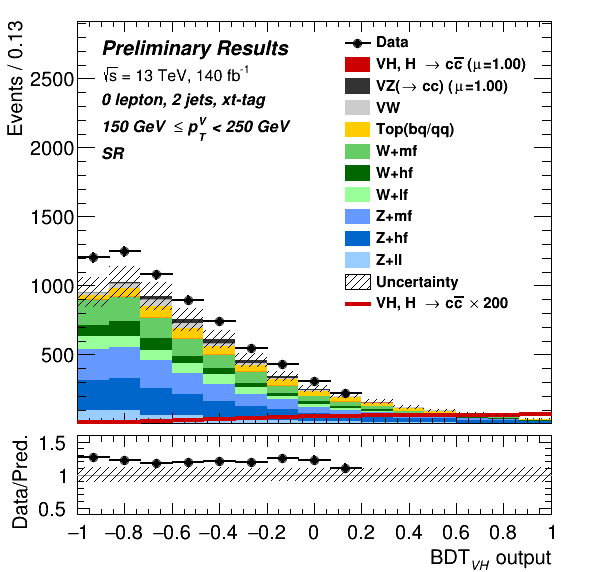
\includegraphics[width=\textwidth]{Images/VH/Own_fit/prefit_VHcc/Region_distmva_BMax250_BMin150_DSR_J2_TTypext_T2_L0_Y6051_Prefit.png}
      \caption{0-lepton, 2-jet.}
      \label{fig:plots_VHcc_ex_OL_SR_2C}
  \end{subfigure}
  \begin{subfigure}[b]{0.32\textwidth}
      \centering
      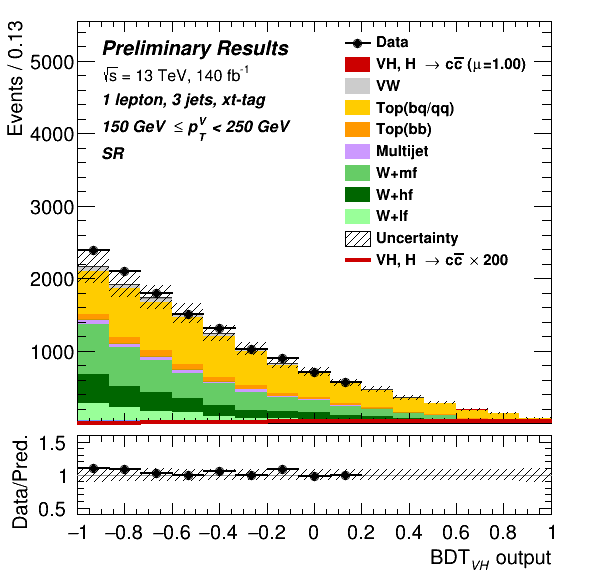
\includegraphics[width=\textwidth]{Images/VH/Own_fit/prefit_VHcc/Region_distmva_BMax250_BMin150_DSR_J3_TTypext_T2_L1_Y6051_Prefit.png}
      \caption{1-lepton, 3-jet.}
      \label{fig:plots_VHcc_ex_1L_SR_2C}
  \end{subfigure}
  \begin{subfigure}[b]{0.32\textwidth}
    \centering
    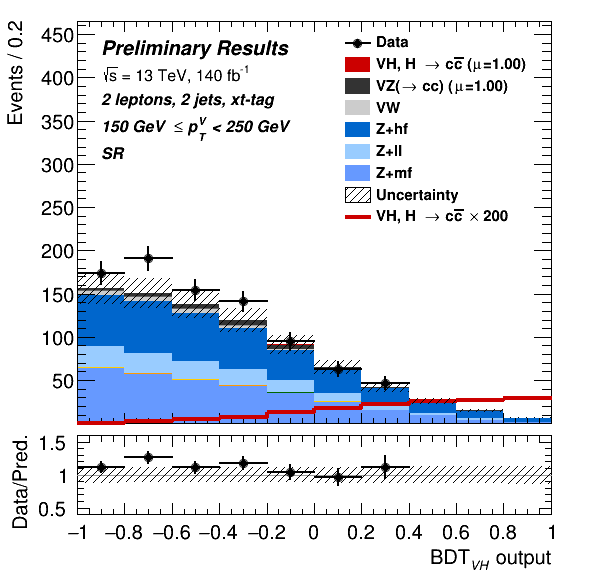
\includegraphics[width=\textwidth]{Images/VH/Own_fit/prefit_VHcc/Region_distmva_BMax250_BMin150_DSR_J2_TTypext_T2_L2_Y6051_Prefit.png}
    \caption{2-lepton, 2-jet.}
    \label{fig:plots_VHcc_ex_2L_SR_2C}
\end{subfigure}
  \caption{Selection of 2 $c$-tagged ($TT$ + $LT$) 150 < \ptv\ < 250 GeV signal regions.}
  \label{fig:plots_VHcc_ex_SR_2C}
\end{figure} 


\begin{figure}[h!]
  \centering
  \begin{subfigure}[b]{0.32\textwidth}
      \centering
      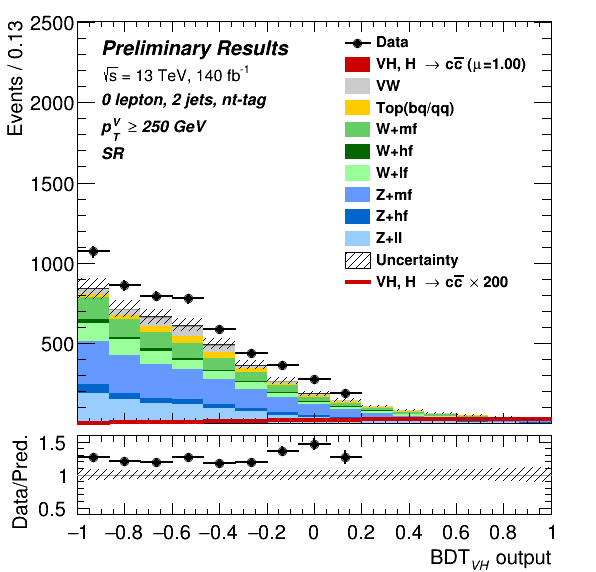
\includegraphics[width=\textwidth]{Images/VH/Own_fit/prefit_VHcc/Region_distmva_BMin250_DSR_J2_TTypent_T1_L0_Y6051_Prefit.png}
      \caption{0-lepton, 2-jet.}
      \label{fig:plots_VHcc_ex_OL_SR_1C}
  \end{subfigure}
  \begin{subfigure}[b]{0.32\textwidth}
      \centering
      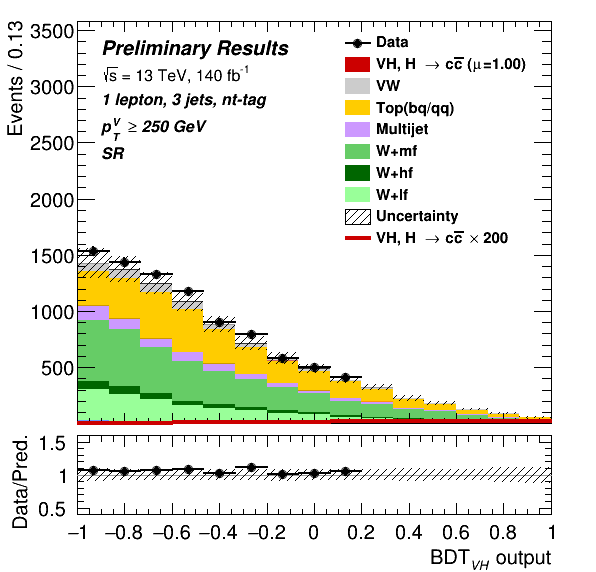
\includegraphics[width=\textwidth]{Images/VH/Own_fit/prefit_VHcc/Region_distmva_BMin250_DSR_J3_TTypent_T1_L1_Y6051_Prefit.png}
      \caption{1-lepton, 3-jet.}
      \label{fig:plots_VHcc_ex_1L_SR_1C}
  \end{subfigure}
  \begin{subfigure}[b]{0.32\textwidth}
    \centering
    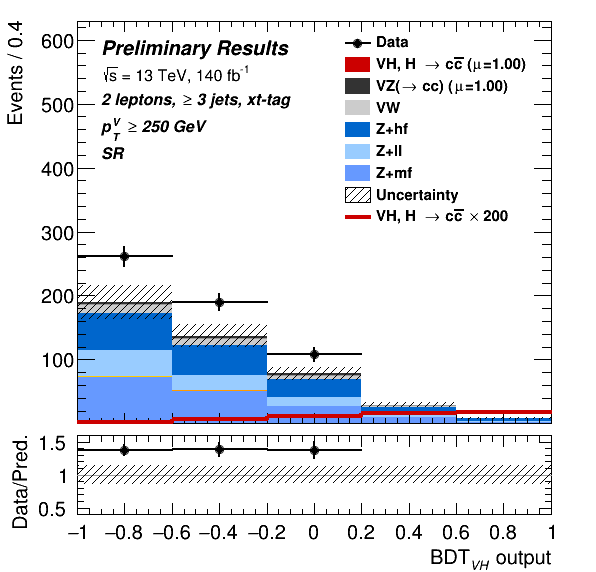
\includegraphics[width=\textwidth]{Images/VH/Own_fit/prefit_VHcc/Region_distmva_BMin250_DSR_J3_TTypext_incJet1_T2_L2_Y6051_Prefit.png}
    \caption{2-lepton, $\geq$ 3 (3p) jets.}
    \label{fig:plots_VHcc_ex_2L_SR_1C}
\end{subfigure}
  \caption{Selection of 1 $c$-tagged 250 < \ptv\ signal regions.}
  \label{fig:plots_VHcc_ex_SR_1C}
\end{figure} 

\paragraph{The High $\Delta R$ Control Regions:} are designed for the resolved regime to constrain the normalisation and shape of the $V+$jets and the \ttb\ background when the 2 candidate jets are the $b$-quarks. They are defined by a further split from the \glspl{sr} based on the angular separation $\Delta R(j_1, j_2)$\footnote{$\Delta R(j_1, j_2) = \sqrt{(\eta_{j_1} - \eta_{j_2})^2 + (\phi_{j_1} - \phi_{j_2})^2 }$.} (shortened as $\Delta R$ in this document) between the Higgs-candidate jets. This split is governed by a $p_T^V$-dependent cut on the $\Delta R$ that is derived to give a specific signal purity in the \gls{sr}: keeping 95\% (85\%) of the signal yield in the 2-jet (3 or more jets) \glspl{sr}. The mathematical expression of the cuts is presented in Table \ref{tbl:CRhigh_definition}, and illustrated in Figure~\ref{fig:drccptvCutsVHcc}, with more details given in Appendix~\ref{ap-sec-vh-deltaR}. Events with a $\Delta R$ below the cutting line enter the signal region, while those above go in a \highdr\ \gls{cr}, also called \textit{CRHigh}. To avoid some mis-modelling effect at high $\Delta R$ and keep the \highdr\ \gls{cr} kinematically close to the \gls{sr}, an uppercut of $\Delta R \leq \pi$ is applied to all events. This effectively removes $\sim 40$\% of events in the \highdr\ \gls{cr}, with a negligible impact on the signal region. For \vhc, CRHighs are considered for every 1 and 2 $c$-tagged \glspl{sr}\footnote{Also for the in the 1L-channel in the 1 $c$-tagged 75 GeV $<$ \ptv\ $<$ 150 GeV, where the equivalent SR is not included.}, with the $TT$- and $LT$-tagged events separated in the CRHigh to respectively constrain the \vhf\ and \vmf instead of being merged as in the \gls{sr}. In \vhb, the CRHighs are used to extract the normalisation of the backgrounds while in \vhc\ the shapes of the $m_{c\bar{c}}$ and \ptv\ spectrum are also used, as detailed in Section~\ref{sec-vh-disc}. Some \highdr\ \glspl{cr} are shown in Figure~\ref{fig:plots_VHcc_ex_CRH}.

\begin{table}[htbp]
    \centering
    \begin{tabular}{c|c|c}
      \hline
      \hline
      Category & \highdr\ Cut & \lowdr\ Cut\\ \hline
      $2$-jet & $ \Delta R > 0.787 + e^{1.387 - 0.0070 \times p_{T}^{V} } $      &  $ \Delta R < 0.410 + e^{ 0.818 - 0.0106  \times p_{T}^{V} } $        \\
      $3$-jet & $ \Delta R > 0.684 + e^{1.204 - 0.0060 \times p_{T}^{V} } $      &  $ \Delta R < 0.430 + e^{ 0.399 - 0.0093  \times p_{T}^{V} } $        \\
      $4$-jet & $ \Delta R > 0.863 + e^{0.984 - 0.0041 \times p_{T}^{V} } $ &  $ \Delta R < 0.411 + e^{ 1.204 - 0.0060  \times p_{T}^{V} } $        \\
      $\geq$5-jet & $ \Delta R > 1.667 + e^{0.519 - 0.0050 \times p_{T}^{V} } $ &  $ \Delta R < 0.501 + e^{ 1.192 - 0.0075  \times p_{T}^{V} } $      \\
      \hline
      \hline
    \end{tabular}
    \caption{Cuts defining the \highdr\ (centre) and \lowdr\ (right) control regions, CRHigh \& CRLow. The inequalities are set to enter the control regions, with \ptv\ expressed in GeV.}
    \label{tbl:CRhigh_definition}
  \end{table} % TODO: units of \ptv ???
  
\begin{figure}[h!]
    %\hspace{-2.0cm}
    \center
    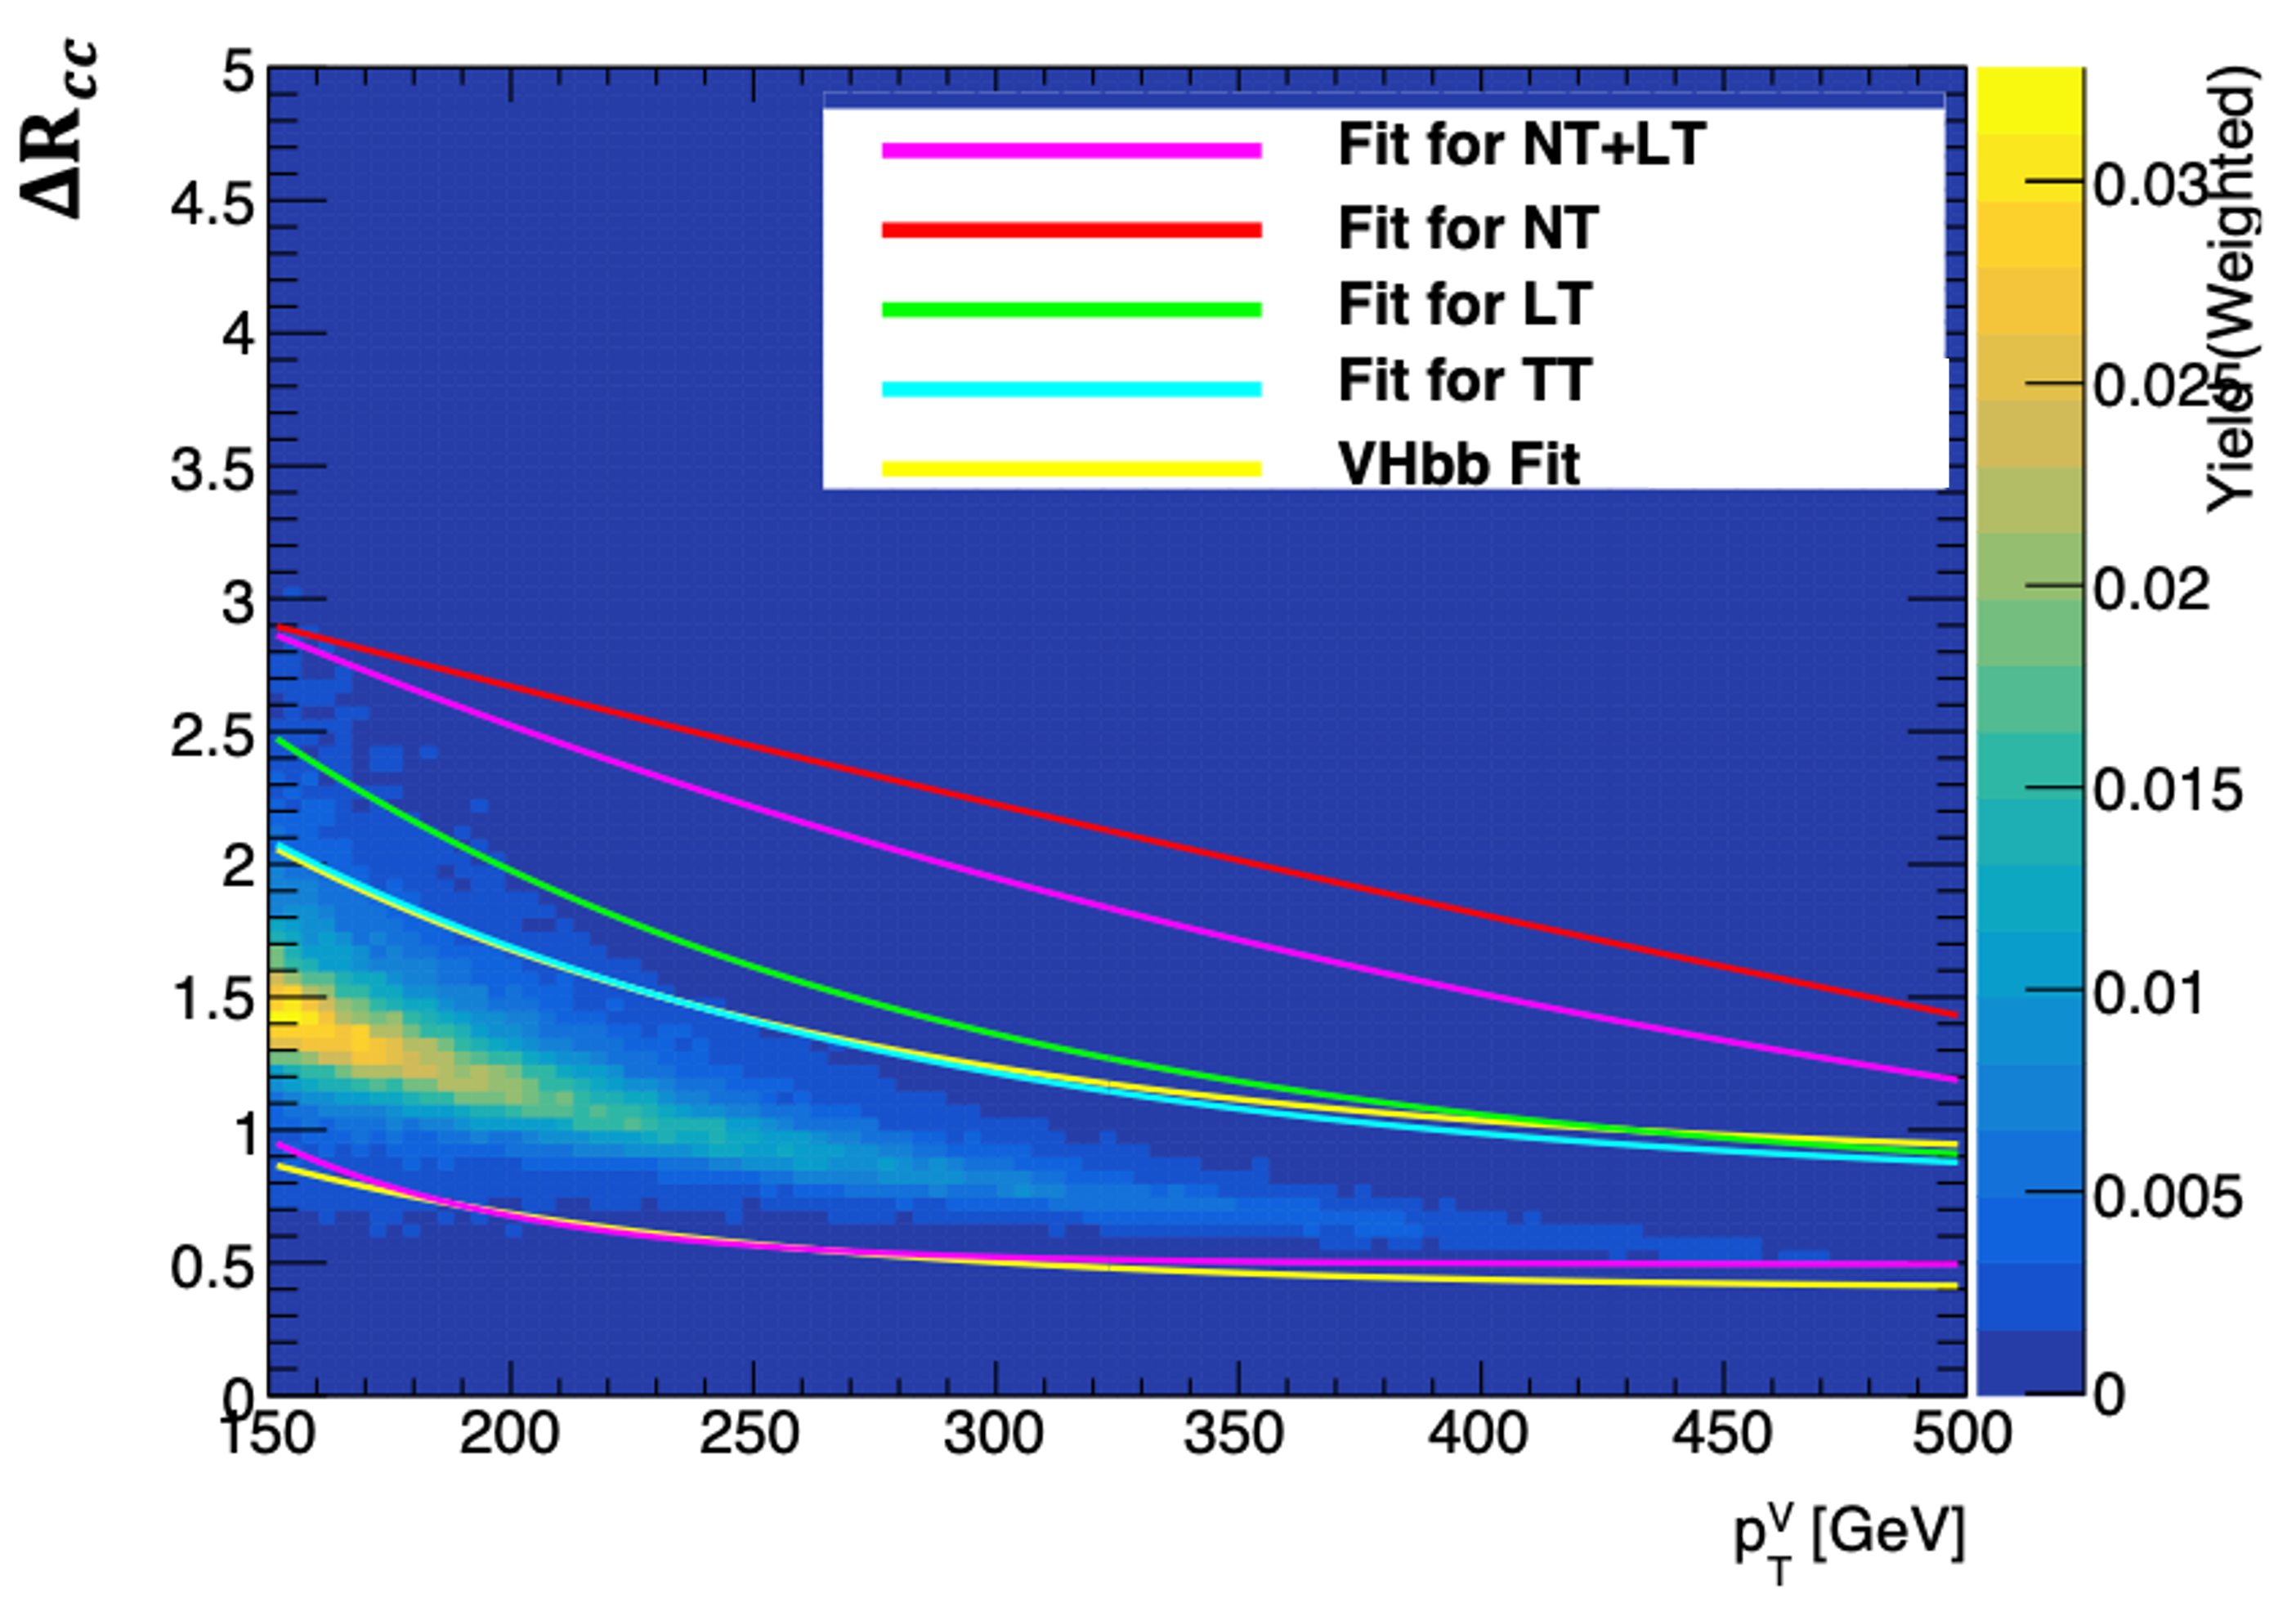
\includegraphics[width=0.48\textwidth]{Images/VH/dRccpTV/sr1.png}
    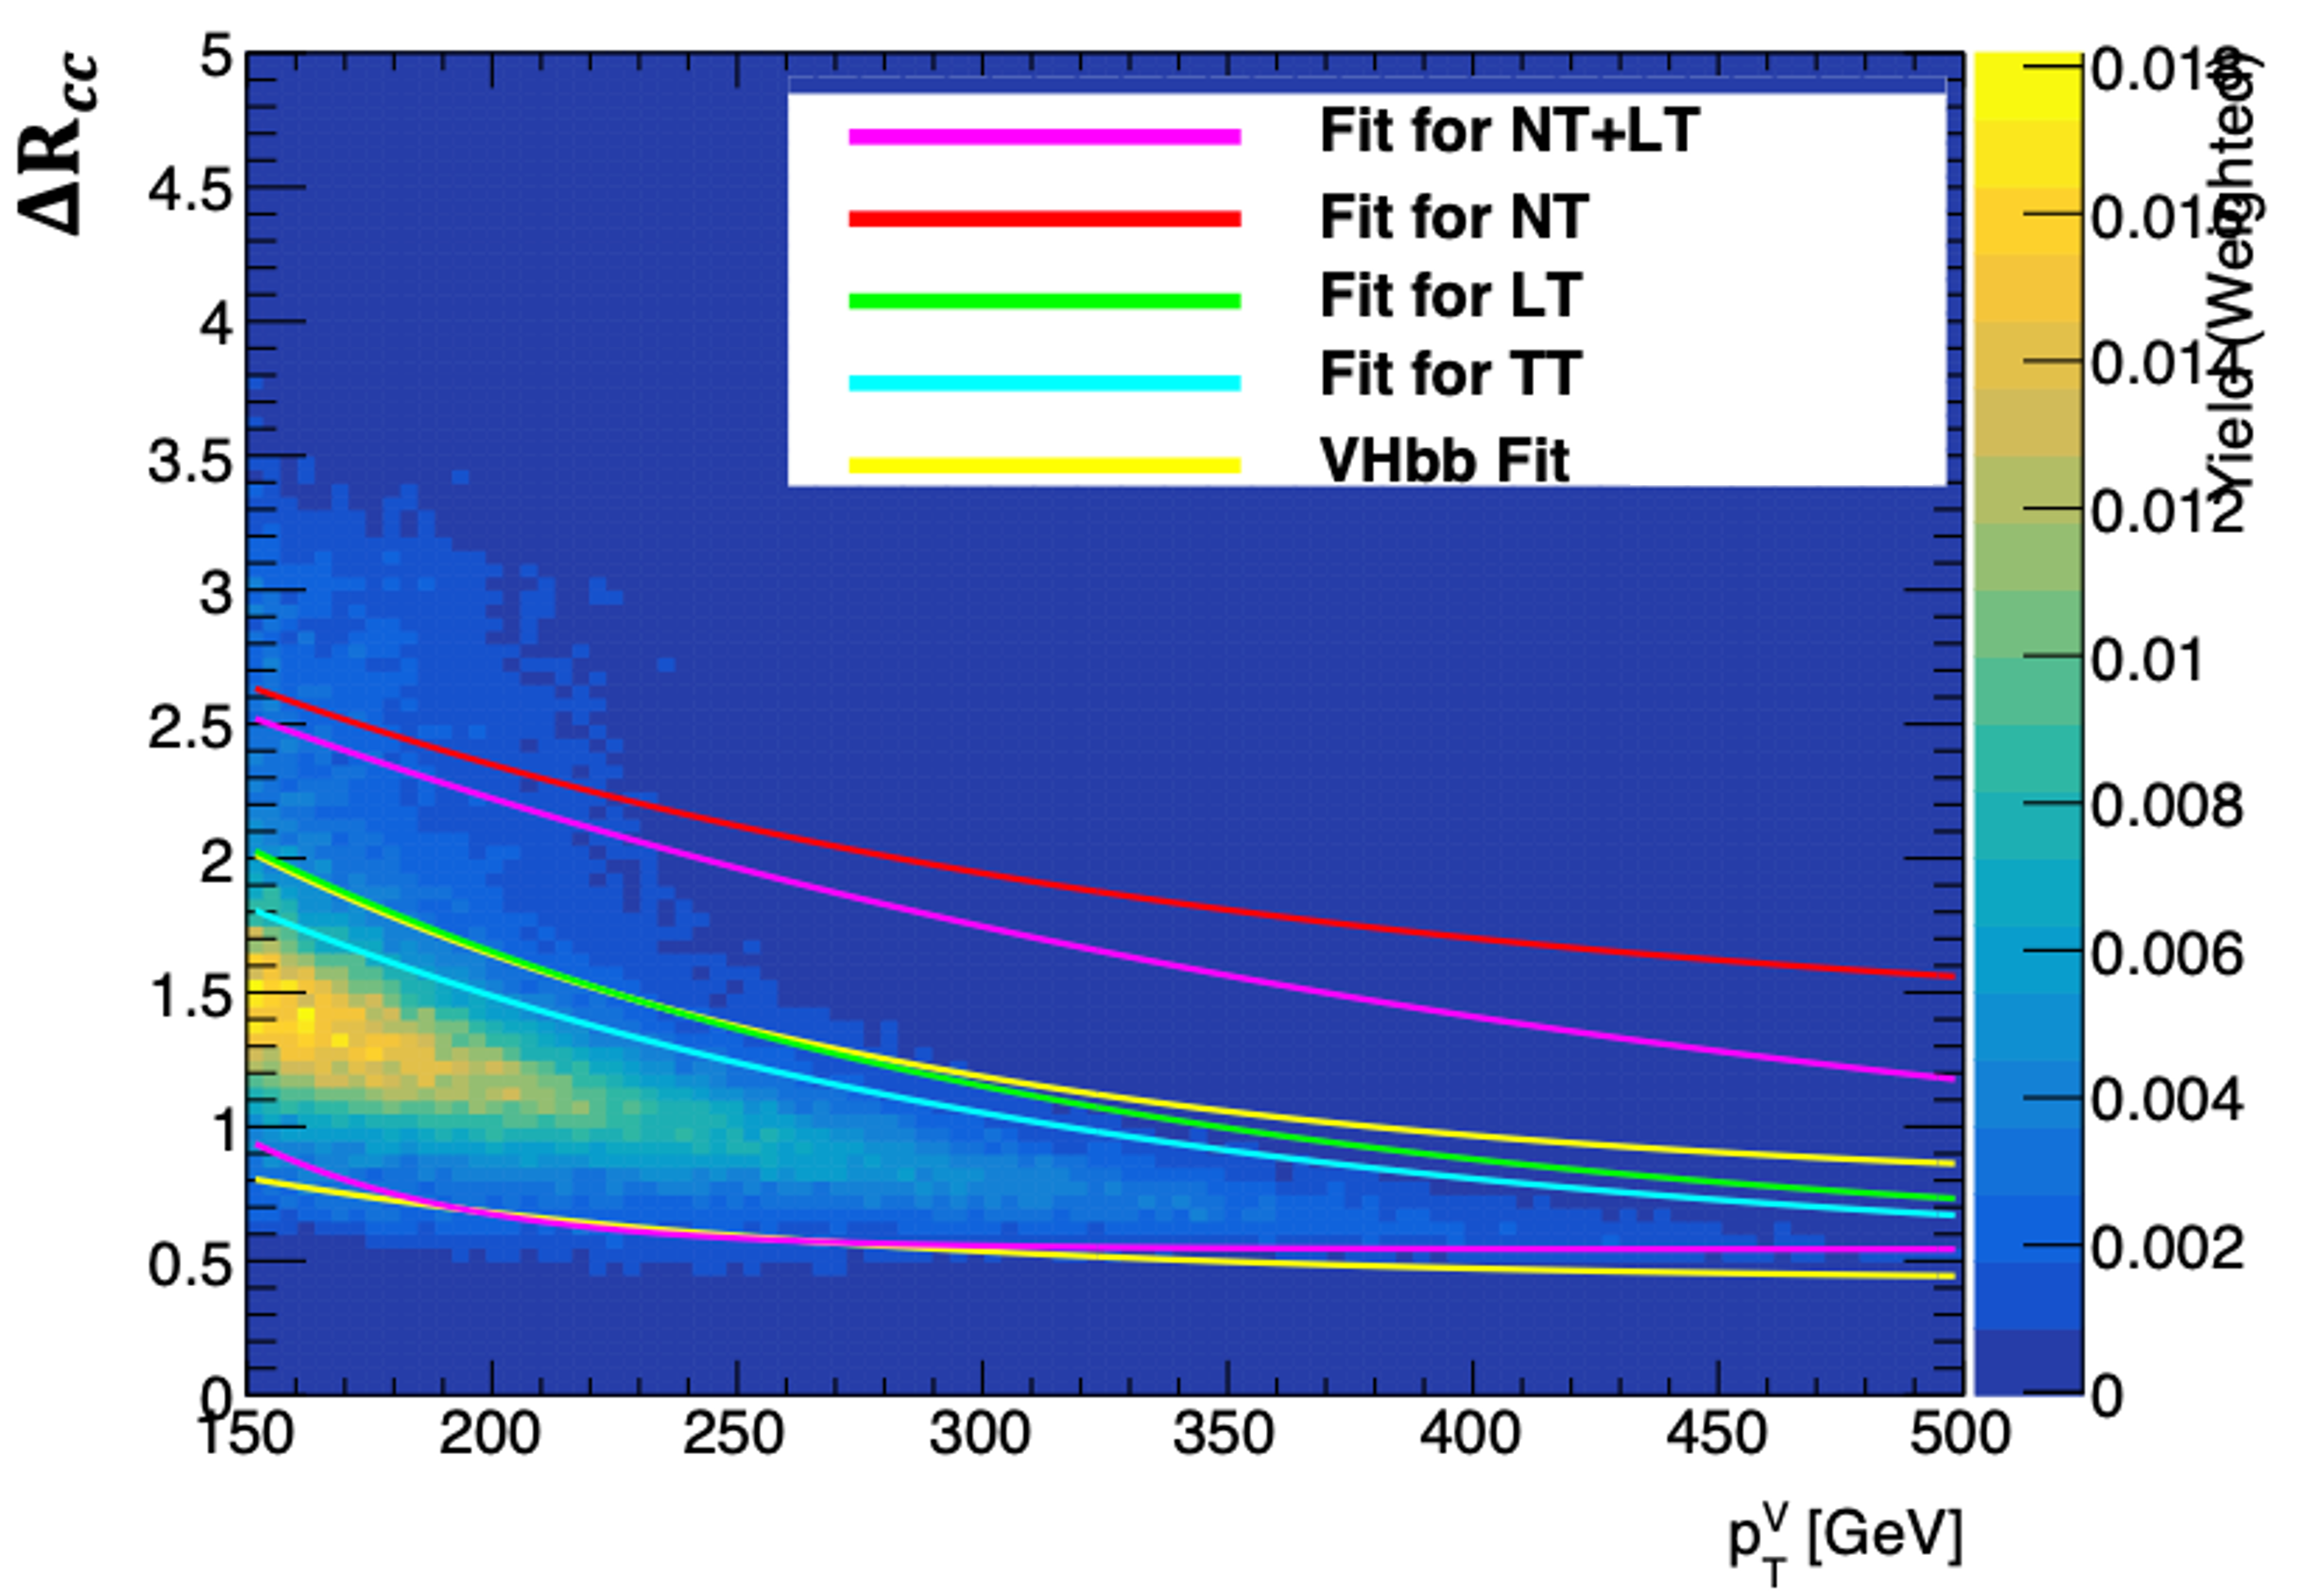
\includegraphics[width=0.48\textwidth]{Images/VH/dRccpTV/sr2.png}
    \caption{The $p_T^V$-$\Delta R_{c\bar{c}}$ 2D signal yield map of the 1-lepton \vhc, for the 2-jet (left) and 3-jet (right) regions. The lines are the results of fitting the high and low $\Delta R_{c\bar{c}}(p_T^V)$ cuts for various signal tags, with the yellow curve showing the \vhb\ $\Delta R_{b\bar{b}}$ cut used in the analysis, with the CRHigh above the top yellow line, and the SR below. A \lowdr\ CR can be defined by the bottom lines, splitting an extra region from the signal region for the \vhb\ only.} 
    \label{fig:drccptvCutsVHcc}
\end{figure}

\begin{figure}[h!]
  \centering
  \begin{subfigure}[b]{0.32\textwidth}
      \centering
      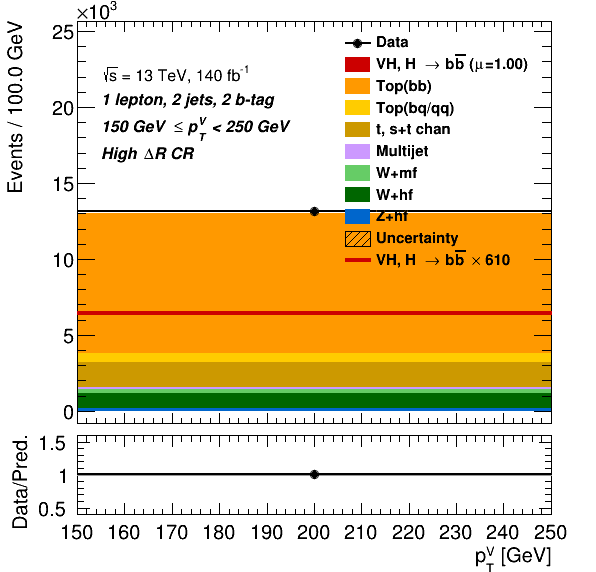
\includegraphics[width=\textwidth]{Images/VH/Own_fit/prefit_VHbb/Region_distpTV_BMax250_BMin150_DCRHigh_J2_TTypebb_T2_L1_Y6051_Prefit.png}
      \caption{1-lepton, $BB$.}
      \label{fig:plots_VHcc_ex_OL_CRH}
  \end{subfigure}
  \begin{subfigure}[b]{0.32\textwidth}
      \centering
      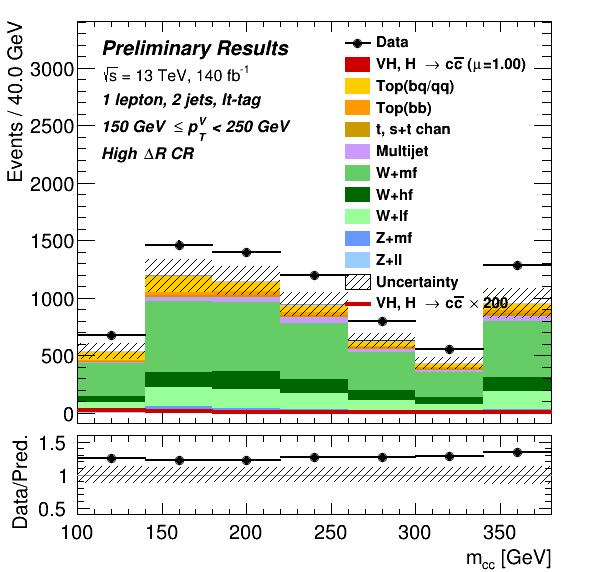
\includegraphics[width=\textwidth]{Images/VH/Own_fit/prefit_VHcc/Region_distmBB_BMax250_BMin150_DCRHigh_J2_TTypelt_T2_L1_Y6051_Prefit.png}
      \caption{1-lepton $LT$.}
      \label{fig:plots_VHcc_ex_1L_CRH}
  \end{subfigure}
  \begin{subfigure}[b]{0.32\textwidth}
    \centering
    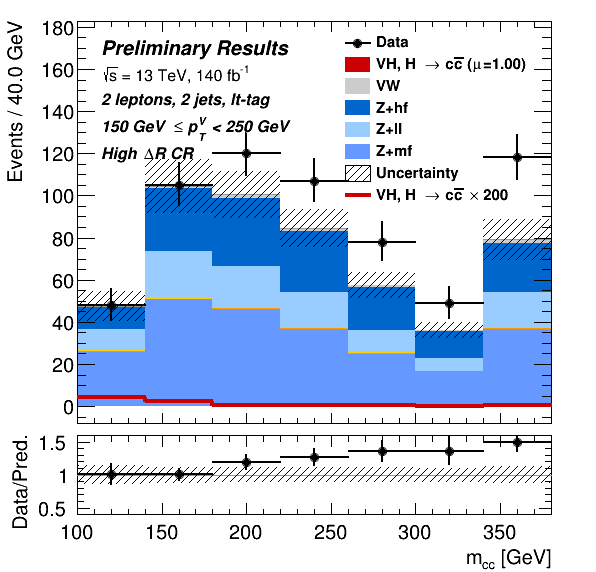
\includegraphics[width=\textwidth]{Images/VH/Own_fit/prefit_VHcc/Region_distmBB_BMax250_BMin150_DCRHigh_J2_TTypelt_T2_L2_Y6051_Prefit.png}
    \caption{2-lepton $LT$.}
    \label{fig:plots_VHcc_ex_2L_CRH}
\end{subfigure}
  \caption{Some \highdr\ \glspl{cr} (CRHigh) with 2 jets and 150 < \ptv\ < 250 GeV.}
  \label{fig:plots_VHcc_ex_CRH}
\end{figure} 

\paragraph{The Low $\Delta R$ Control Regions:} low-$\Delta R$ control regions (\textit{CRLow}) are defined in \vhb\ 1L to better constrain the $W+$hf contribution. They are based on \ptv-dependant cuts defined similarly to the \highdr\ ones, separating 10\% of the diboson events from the signal regions, as displayed in the bottom parts of the plots in Figure~\ref{fig:drccptvCutsVHcc}. The cuts used are defined in the right of Table \ref{tbl:CRhigh_definition}, where events with a $\Delta R$ above the cutting line enter the signal region while those below go to the CRLow. In \vhc\ and the 0L and 1L \vhb, the CRLow is not separated from the signal region as it has little impact on the sensitivity of the fit. One of the CRLow regions is presented on the left of Figure~\ref{fig:plots_VH_ex_CRL_CRvl}.

\paragraph{Top Control Regions in 0L and 1L:} are defined to constrain the Top background Top($bc$) and Top($bl$) components\footnote{The component in the parenthesis refers to the flavour of the Higgs-candidate jets. As explained later in this chapter, they are floated together in the fit as the Top$(bq/qq)$.}. The so-called \textit{Top $BT$ CRs} are shared by the resolved \vhb\ and \vhc, with similar \ptv\ and jet multiplicity categorisation as the \glspl{sr}. In 0L and 1L, they are defined by requiring events to have at least one $B$-tag and at least one tight $c$-tag $T$, making them orthogonal to the \vhb\ signal regions. The Higgs candidate is reconstructed from the leading $B$ jet among $B$-tagged jet and leading $T$ jet among $T$-tagged jet, for kinematic similarity to the \glspl{sr}. The Top($bb$) component, which is significant for \vhb\ due to the required tag, is controlled from the previously defined CRHighs in 0L and 1L, thanks to the large $\Delta R$ between the produced $b$ jets in a \ttb, as shown in Figure~\ref{fig:plots_VHcc_ex_OL_CRH}. Two Top $BT$ control regions are presented on the left of Figure~\ref{fig:plots_VHcc_ex_TopCR}.

\begin{figure}[h!]
  \centering
  \begin{subfigure}[b]{0.32\textwidth}
      \centering
      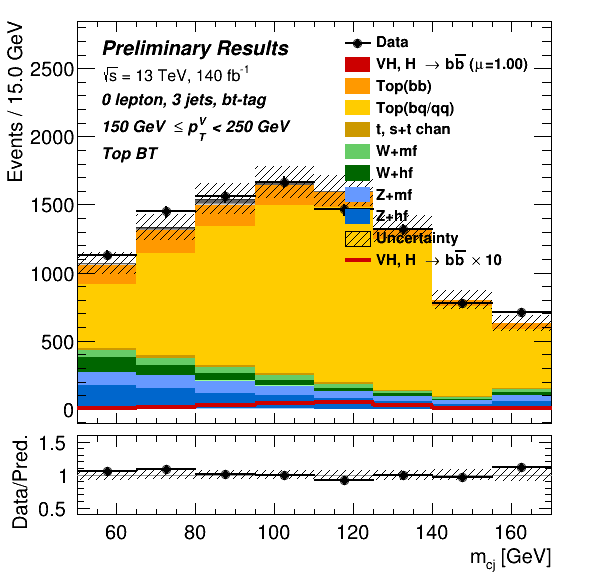
\includegraphics[width=\textwidth]{Images/VH/Own_fit/prefit_VHcc/Region_distmBB_BMax250_BMin150_DtopCRBC_J3_TTypebt_T1_L0_Y6051_Prefit.png}
      \caption{0-lepton, $BT$, 3-jet.}
      \label{fig:plots_VHcc_ex_OL_TopCR}
  \end{subfigure}
  \begin{subfigure}[b]{0.32\textwidth}
      \centering
      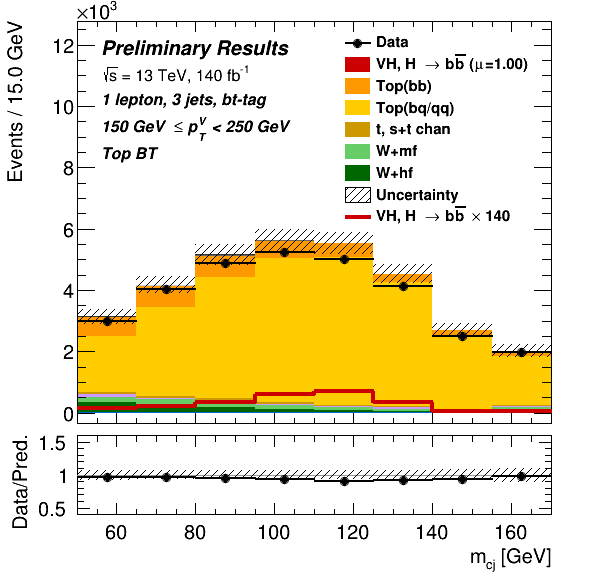
\includegraphics[width=\textwidth]{Images/VH/Own_fit/prefit_VHcc/Region_distmBB_BMax250_BMin150_DtopCRBC_J3_TTypebt_T1_L1_Y6051_Prefit.png}
      \caption{1-lepton, $BT$, 3-jet.}
      \label{fig:plots_VHcc_ex_1L_TopCR}
  \end{subfigure}
  \begin{subfigure}[b]{0.32\textwidth}
    \centering
    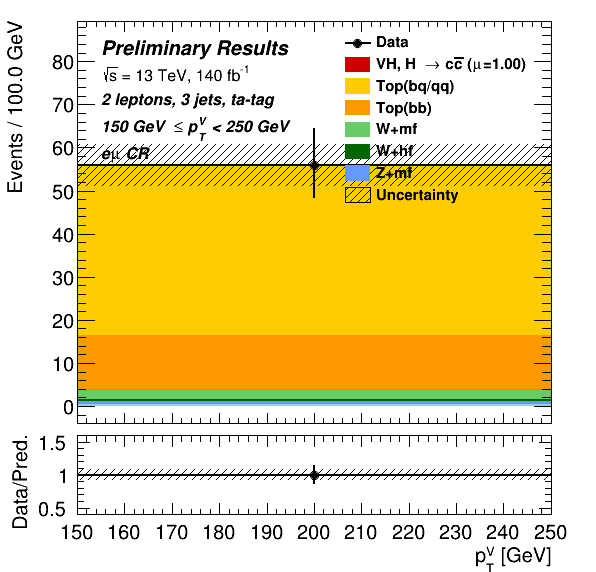
\includegraphics[width=\textwidth]{Images/VH/Own_fit/prefit_VHcc/Region_distpTV_BMax250_BMin150_Dtopemucr_J3_TTypeta_T2_L2_Y6051_Prefit.png}
    \caption{2-lepton, $e\mu$, $\geq$ 1 $T$-tag.}
    \label{fig:plots_VHcc_ex_2L_TopCR}
\end{subfigure}
  \caption{Two Top CR $BT$-tagged (left \& centre) and a Top $e\mu$ CR (right), all with 3 jets and 150 < \ptv\ < 250 GeV.}
  \label{fig:plots_VHcc_ex_TopCR}
\end{figure} 

\paragraph{Top Control Regions in 2L:} there, the Top background is mostly made of di-leptonic \ttb\ decays, with both subsequent $W$ decaying leptonically. High purity Top \glspl{cr} are derived for the 2-lepton channels by requiring leptons of different flavours ($e\mu$ or $\mu e$) instead of the same flavour ($ee$ or $\mu\mu$). This mix of flavours is possible as the leptons are produced in distinct $W$-boson decays. These so-called \textit{Top} $e\mu$ \textit{CRs} are used to derive a \ttb\ background template in a data-driven way for the 2-lepton \glspl{sr} in \vhb. For \vhc, the \ttb\ is a less significant component due to the flavour tagging requirements, and the Top $e\mu$ \glspl{cr} contribute to the fit as single-bin 2-lepton \glspl{cr} per \ptv\ and jet multiplicity, with at least one $T$-tag jet. An example of such a \gls{cr} is presented in Figure~\ref{fig:plots_VHcc_ex_2L_TopCR}.

\begin{figure}[h!]
  \centering
  \begin{subfigure}[b]{0.32\textwidth}
      \centering
      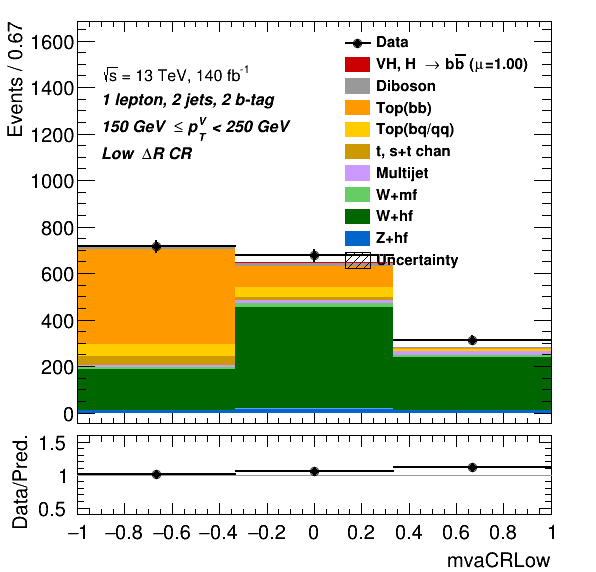
\includegraphics[width=\textwidth]{Images/VH/Own_fit/prefit_VHbb/Region_distmvaCRLow_BMax250_BMin150_DCRLow_J2_TTypebb_T2_L1_Y6051_Prefit.png}
      \caption{1-lepton \lowdr\ CR, $BB$.}
      \label{fig:plots_VHb_ex_1L_CRL}
  \end{subfigure}
  \begin{subfigure}[b]{0.32\textwidth}
      \centering
      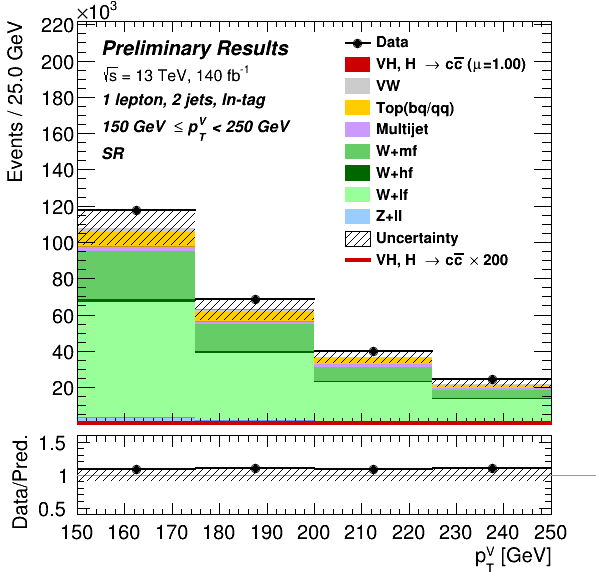
\includegraphics[width=\textwidth]{Images/VH/Own_fit/prefit_VHcc/Region_distpTV_BMax250_BMin150_DSR_J2_TTypeln_T1_L1_Y6051_Prefit.png}
      \caption{1-lepton $V+l$ CR $LN$.}
      \label{fig:plots_VHcc_ex_1L_CRvl}
  \end{subfigure}
  \begin{subfigure}[b]{0.32\textwidth}
    \centering
    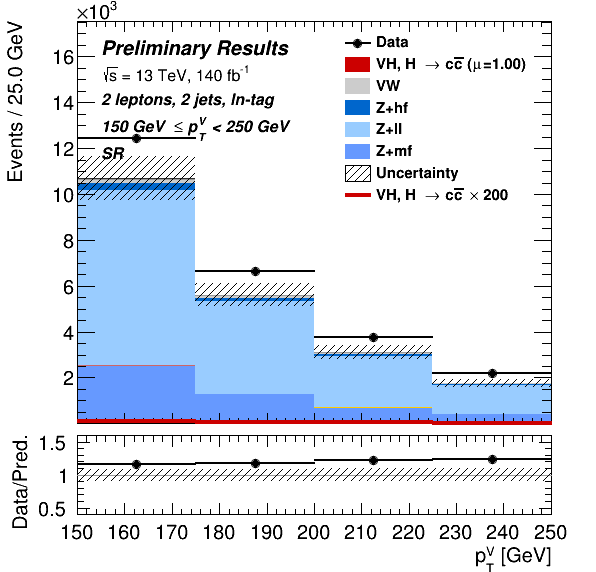
\includegraphics[width=\textwidth]{Images/VH/Own_fit/prefit_VHcc/Region_distpTV_BMax250_BMin150_DSR_J2_TTypeln_T1_L2_Y6051_Prefit.png}
    \caption{2-lepton $V+l$ CR $LN$.}
    \label{fig:plots_VHcc_ex_2L_CRvl}
\end{subfigure}
  \caption{A $BB$-tagged \lowdr\ CR (left) and two $LN$-tagged $V+l$ CRs (centre \& right), both with 2 jets and 150 < \ptv\ < 250 GeV.}
  \label{fig:plots_VH_ex_CRL_CRvl}
\end{figure} 

\paragraph{$V$ $+$ light-jets Control Regions:} the $V$ $+$ light-jets background is particularly significant for \vhc, due to the difficulties in discriminating $c$-jets from light-jets. Dedicated \glspl{cr}, labelled \textit{$V+l$ \gls{cr}}, in the 1L and 2L channels target, respectively, the \wlf\ and \zlf\ backgrounds\footnote{The \vlf\ corresponds to a grouping of the $V+$jets components with light-flavour jets, as introduced in Section~\ref{sec-modVjet}.}. They are defined by requiring exactly one loose $L$-tag $c$-jet without any $T$- nor $B$-tagged jet in the event. The selection is otherwise similar to that of the 1 $c$-tagged signal regions\footnote{Similarly to these SRs, there is no 1L $V+l$ CR for 75 GeV $<$ \ptv\ $<$ 150 GeV.}, with the candidate pair now tagged as $LN$, where $N$ is the leading untagged central jet. The 1L $V+l$ \glspl{cr} are 60\% pure in \wlf, while the 2L $V+l$ \glspl{cr} reach a 70\% \zlf\ purity. An example of the former is shown in Figure~\ref{fig:plots_VHcc_ex_1L_CRvl}, while a 2L $V+l$ \gls{cr} is shown in Figure~\ref{fig:plots_VHcc_ex_2L_CRvl}. 

\begin{figure}[h!]
  \centering
  \begin{subfigure}[b]{0.32\textwidth}
      \centering
      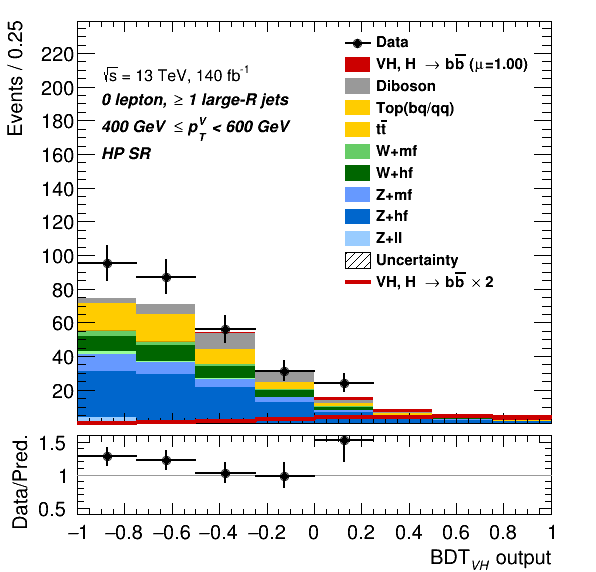
\includegraphics[width=\textwidth]{Images/VH/Own_fit/prefit_VHbb/Region_distmva_BMax600_BMin400_incFat1_Fat1_DSRnoaddbjetsr_J0_TTypebb_T2_L0_Y6051_Prefit.png}
      \caption{0-lepton high purity SR.}
      \label{fig:plots_VHboost_ex_0L_SR}
  \end{subfigure}
  \begin{subfigure}[b]{0.32\textwidth}
      \centering
      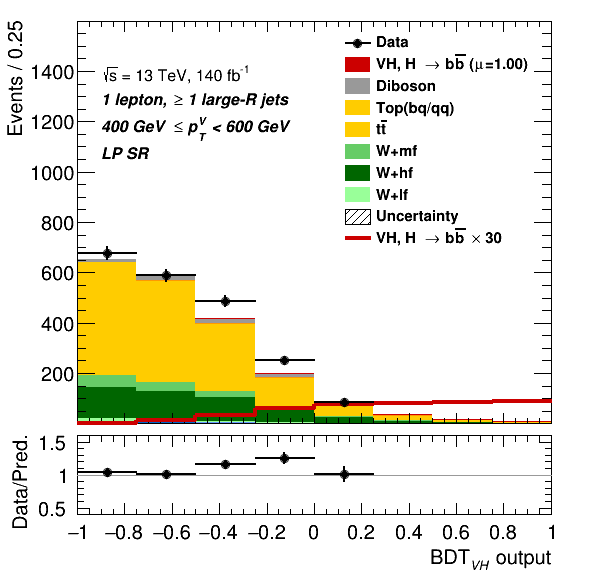
\includegraphics[width=\textwidth]{Images/VH/Own_fit/prefit_VHbb/Region_distmva_BMax600_BMin400_incFat1_Fat1_DSRnoaddbjetsr_J1_TTypebb_incJet1_T2_L1_Y6051_Prefit.png}
      \caption{1-lepton low purity SR.}
      \label{fig:plots_VHboost_ex_1L_SR}
  \end{subfigure}
  \begin{subfigure}[b]{0.32\textwidth}
    \centering
    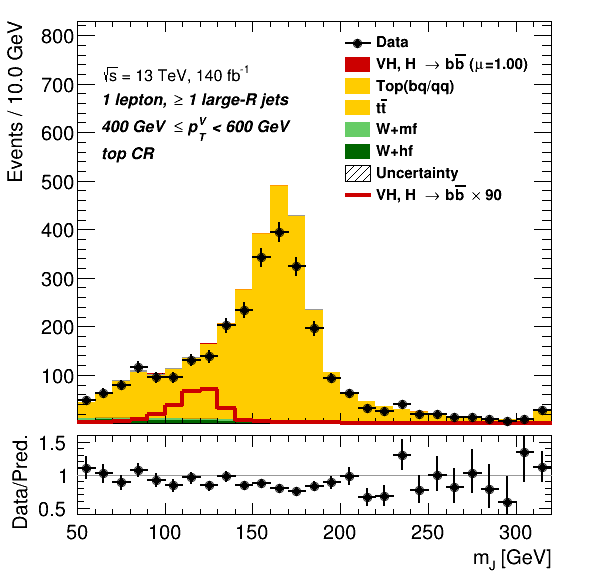
\includegraphics[width=\textwidth]{Images/VH/Own_fit/prefit_VHbb/Region_distmBB_BMax600_BMin400_incFat1_Fat1_DSRtopaddbjetcr_J0_TTypebb_incJet1_T2_L1_Y6051_Prefit.png}
    \caption{1-lepton top CR.}
    \label{fig:plots_VHboost_ex_1L_top}
\end{subfigure}
  \caption{Some boosted $BB$-tagged with 400 < \ptv\ < 600 GeV regions signal regions (left \& centre) and boosted Top CR (right).}
  \label{fig:plots_VHboost_ex}
\end{figure} 

\subsubsection{Boosted Regime Categorisation}
In the boosted \vhb, two \ptv\ bins are defined at [400, 600] GeV and $\geq$ 600 GeV to avoid overlap with the resolved \vhb. The \glspl{sr} are defined by requiring exactly two of the three leading subjets (track-jets) associated with a single leading large-$R$ jet to be $b$-tagged, with no additional track-jet outside the large-$R$ jet being $B$-tagged to enhance the top background rejection. All boosted regions, with processes normalised to their postfit expectations, are presented in Appendix Section~\ref{appsec-vh-analRegBooPosfit}. In the plots, the \glspl{sr} are further separated into a high- (HP) and low-purity, \textit{HP SR} and \textit{LP SR}, when there are no or $\geq$ 1 additional small-$R$ jet not associated to the Higgs-candidate large-$R$ jet. These regions are however combined into single signal regions in the final fit.

\paragraph{Boosted Top Control Regions in 0L and 1L:} events that have an additional $B$-tagged track-jet outside the large-$R$ jet as defined by an angular separation of \[\Delta R(\textrm{VR-track jet, large-}R\textrm{ jet}) > 1\] are moved to the boosted Top control regions in the 0L and 1L channels. The \ttb\ process is the main background in these lepton channels, where a $t$-quark decay is captured as a single large-$R$ jet merging the produced $b$ and a hadronically decaying $W$. The boosted Top \glspl{cr} effectively capture this signature by identifying the $b$-quark from the other decaying $t$-quark in the \ttb\ pair, with the same 85\% $b$-tagging \gls{wp}. An example of such a region is displayed in Figure~\ref{fig:plots_VHboost_ex}.\\

\newpage

\begin{sidewaysfigure}[t!]
    \centering
    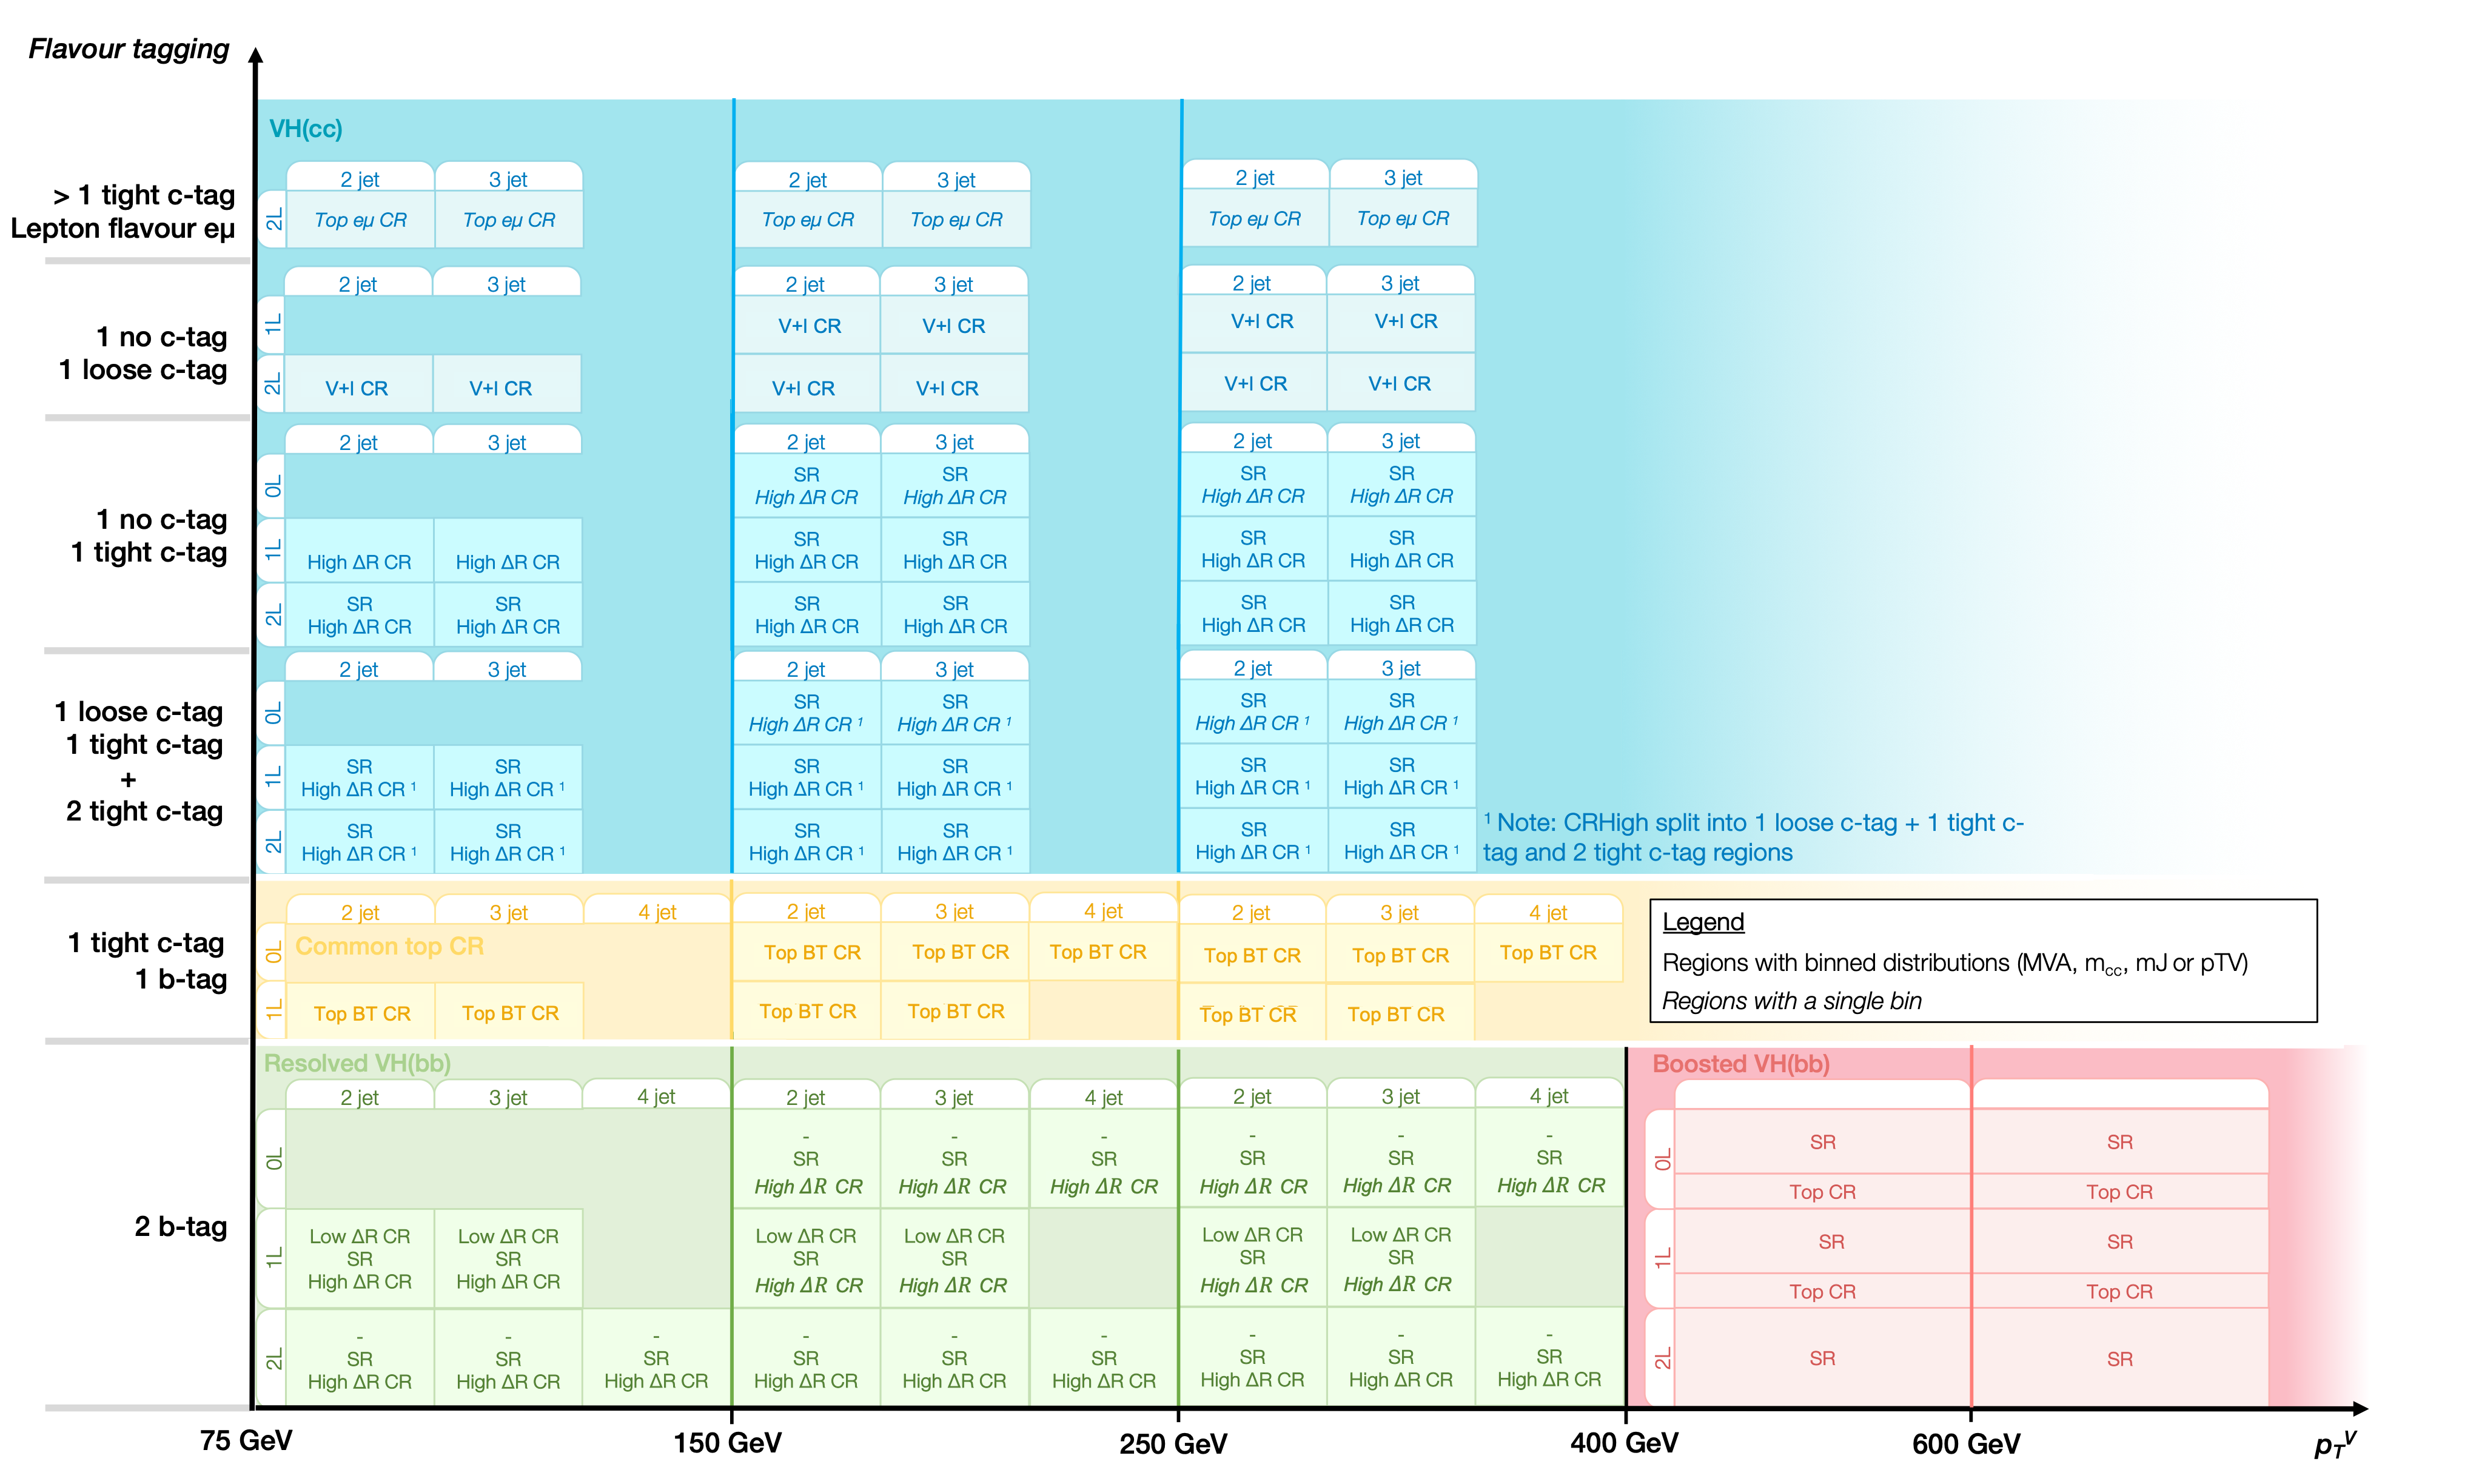
\includegraphics[width=\textwidth]{Images/VH/Cat/VH_analysis_catCorr.png}
    \caption{The \vhbc\ combined analysis regions, showing the Signal Regions (SR), High and Low $\Delta R$ control regions (CRHigh \& LowCR), the Top $BT$ CR, the Top $e\mu$ CR, the $V+l$ $LN$-tagged CR, and the boosted Top CR. \vhc\ is in blue, the shared Top $BT$ CR in the resolved regime in yellow, and \vhb\ in green and red for the resolved and boosted regimes respectively. Regions used in the fit as single-bin distributions to derive an absolute normalisation are indicated in italics. } 
    \label{fig:ana-strat-det}
\end{sidewaysfigure} % TODO: the italic convention is not respected

\clearpage

\section{Tagged-jets Corrections}\label{sec-vh-jetcor}
Several corrections to the energy are applied to tagged jets from the previously introduced selection. The objective is to improve the energy resolution of the pair of jets selected to form the Higgs candidate. All jets benefit from a default jet energy calibration called the \textit{Global Sequential Calibration (GSC)} \cite{PhysRevD.96.072002}, as introduced in Section~\ref{}. This global correction is not optimal for $b$- and $c$-jets that benefit from special features, motivating the use of additional dedicated corrections for such jets. Table \ref{tab:bjetcorrectionregions} summarises the additional corrections presented in this section. % TODO Add a ref to exp chapter, jet section

\begin{table}[!htbp]
  \begin{center}
  \resizebox{\textwidth}{!}{
    \begin{tabular}{c|c|cccc} \hline \hline
      Scheme & Lepton channel & Muon-in-jet & $p_T$-Reco & Kinematic fit & FSR Recovery     \\
      \hline
        \multirow{3}{*}{Resolved \vhb} & 0L & \checkmark & \checkmark &    & \\
                                      & 1L & \checkmark & \checkmark &    & \\  
                                      & 2L & \checkmark & \checkmark (\nj\ $\geq$ 4) & \checkmark (\nj\ $\leq$ 3) & \checkmark (\nj\ $\leq$ 4) \\  
      \hline
        \multirow{3}{*}{\vhc} & 0L & \checkmark &  &    & \\
                                      & 1L & \checkmark &  &    & \\  
                                      & 2L & \checkmark &  & \checkmark (\nj\ $\leq$ 3) & \checkmark (\nj\ $\leq$ 4) \\  
      \hline
        \multirow{3}{*}{boosted \vhb}  & 0L & \checkmark &  &    & \\
                                      & 1L & \checkmark &  &    & \\  
                                      & 2L & \checkmark &  &  \checkmark  & \\  

      \hline \hline
    \end{tabular}
  }
  \caption{The different $H$-candidate jet energy correction.} 
  \label{tab:bjetcorrectionregions}
  \end{center}
\end{table}
  
\paragraph{\textit{Muon-in-jet} correction} is applied to all events to correct the energy of semi-leptonically decaying $b$- and $c$-jets with a muon in the jet cone. The energy of this $\mu$ is not measured in the calorimeter but is deduced from the curvature of the muon track. For the resolved regime, the closest muon's 4-momentum $p_T^{\mu}$ is added to the jet if its angular separation from the jet axis satisfies \[\Delta R(\textrm{jet}, \mu) \leq \min\left(0.4, \,0.04 + \frac{10 \textrm{ GeV}}{p_T^{\mu}}\right).\] In the boosted scheme, the angular separation is measured with respect to the track-jets but the muon 4-momentum $p_T^{\mu}$ is added to the large-$R$ jet in case of a match.

\paragraph{\textit{PtReco} correction} accounts for missing energy from neutrinos in the semi-leptonic decays or from the out-of-cone effect for $b$-jets. It is only applied to $b$-tagged jets in the resolved \vhb\ 0L and 1L channels, and the $\geq4$-jets 2L channel. The correction is derived from the signal samples of \vhb\ by comparing the truth jet $p_T$ and the reconstructed $p_T$ after the muon-in-jet correction. The correction is not applied to \vhc\ as it does not have a significant effect due to the lower likelihood of semi-leptonic decays and out-of-cone effects for $c$-jets.

\paragraph{\textit{Kinematic} fit correction} is applied in the 2L channel of the resolved regime, for events with 2 or 3 jets only. The $ZH \rightarrow\ell\ell b\bar{b} /\ell\ell c\bar{c}$ is fully reconstructed and a kinematic fit is applied to improve the $m_{jj}$ resolution after the muon-in-jet correction. The fit is performed using a likelihood function with terms covering the object resolution, the jet transfer function, a $Z$-mass constraint term, and system $p_T$ balance. The boosted 2L channel has a similar kinematic fit based on a Gaussian term instead. The procedure is not applied to events with more than 3 jets as the benefits are smeared out by the additional jets. % TODO not clear for boosted. % NOTE not passed to the ETmiss.

\paragraph{FSR recovery} is deployed for events with 3 or 4 jets in the 2L resolved regime, to further improve the resolution of the $m_{bb}$ or $m_{cc}$ peak after the kinematic fit correction. Such events are likely to have jets emanating as \glsfirst{fsr}, whereby a quark or a gluon is emitted by a final state particle. A continuous cut on the sum $\Delta R_{j, j_1} + \Delta R_{j, j_2}$ of angular separations between a third or fourth jet ($j$) to the Higgs-candidate jets ($j_1$ and $j_2$) is applied as a function of \ptv. Any additional jet below the cut is considered as a radiation and is added to the closest candidate jet. This effectively corrects the reconstructed mass of Higgs bosons as well as the jet multiplicity, leading to an expected 7\% improvement in \vhb\ \gls{stxs} sensitivity by reducing the migration between measurement bins. Due to the possible increased acceptance of the \ttb\ background in the sensitive region from the reduction of additional jets, this correction is not applied to 0L or 1L.

\begin{figure}[h!]
  %\hspace{-4.0cm}
  \centering
  \begin{subfigure}[b]{0.49\textwidth}
    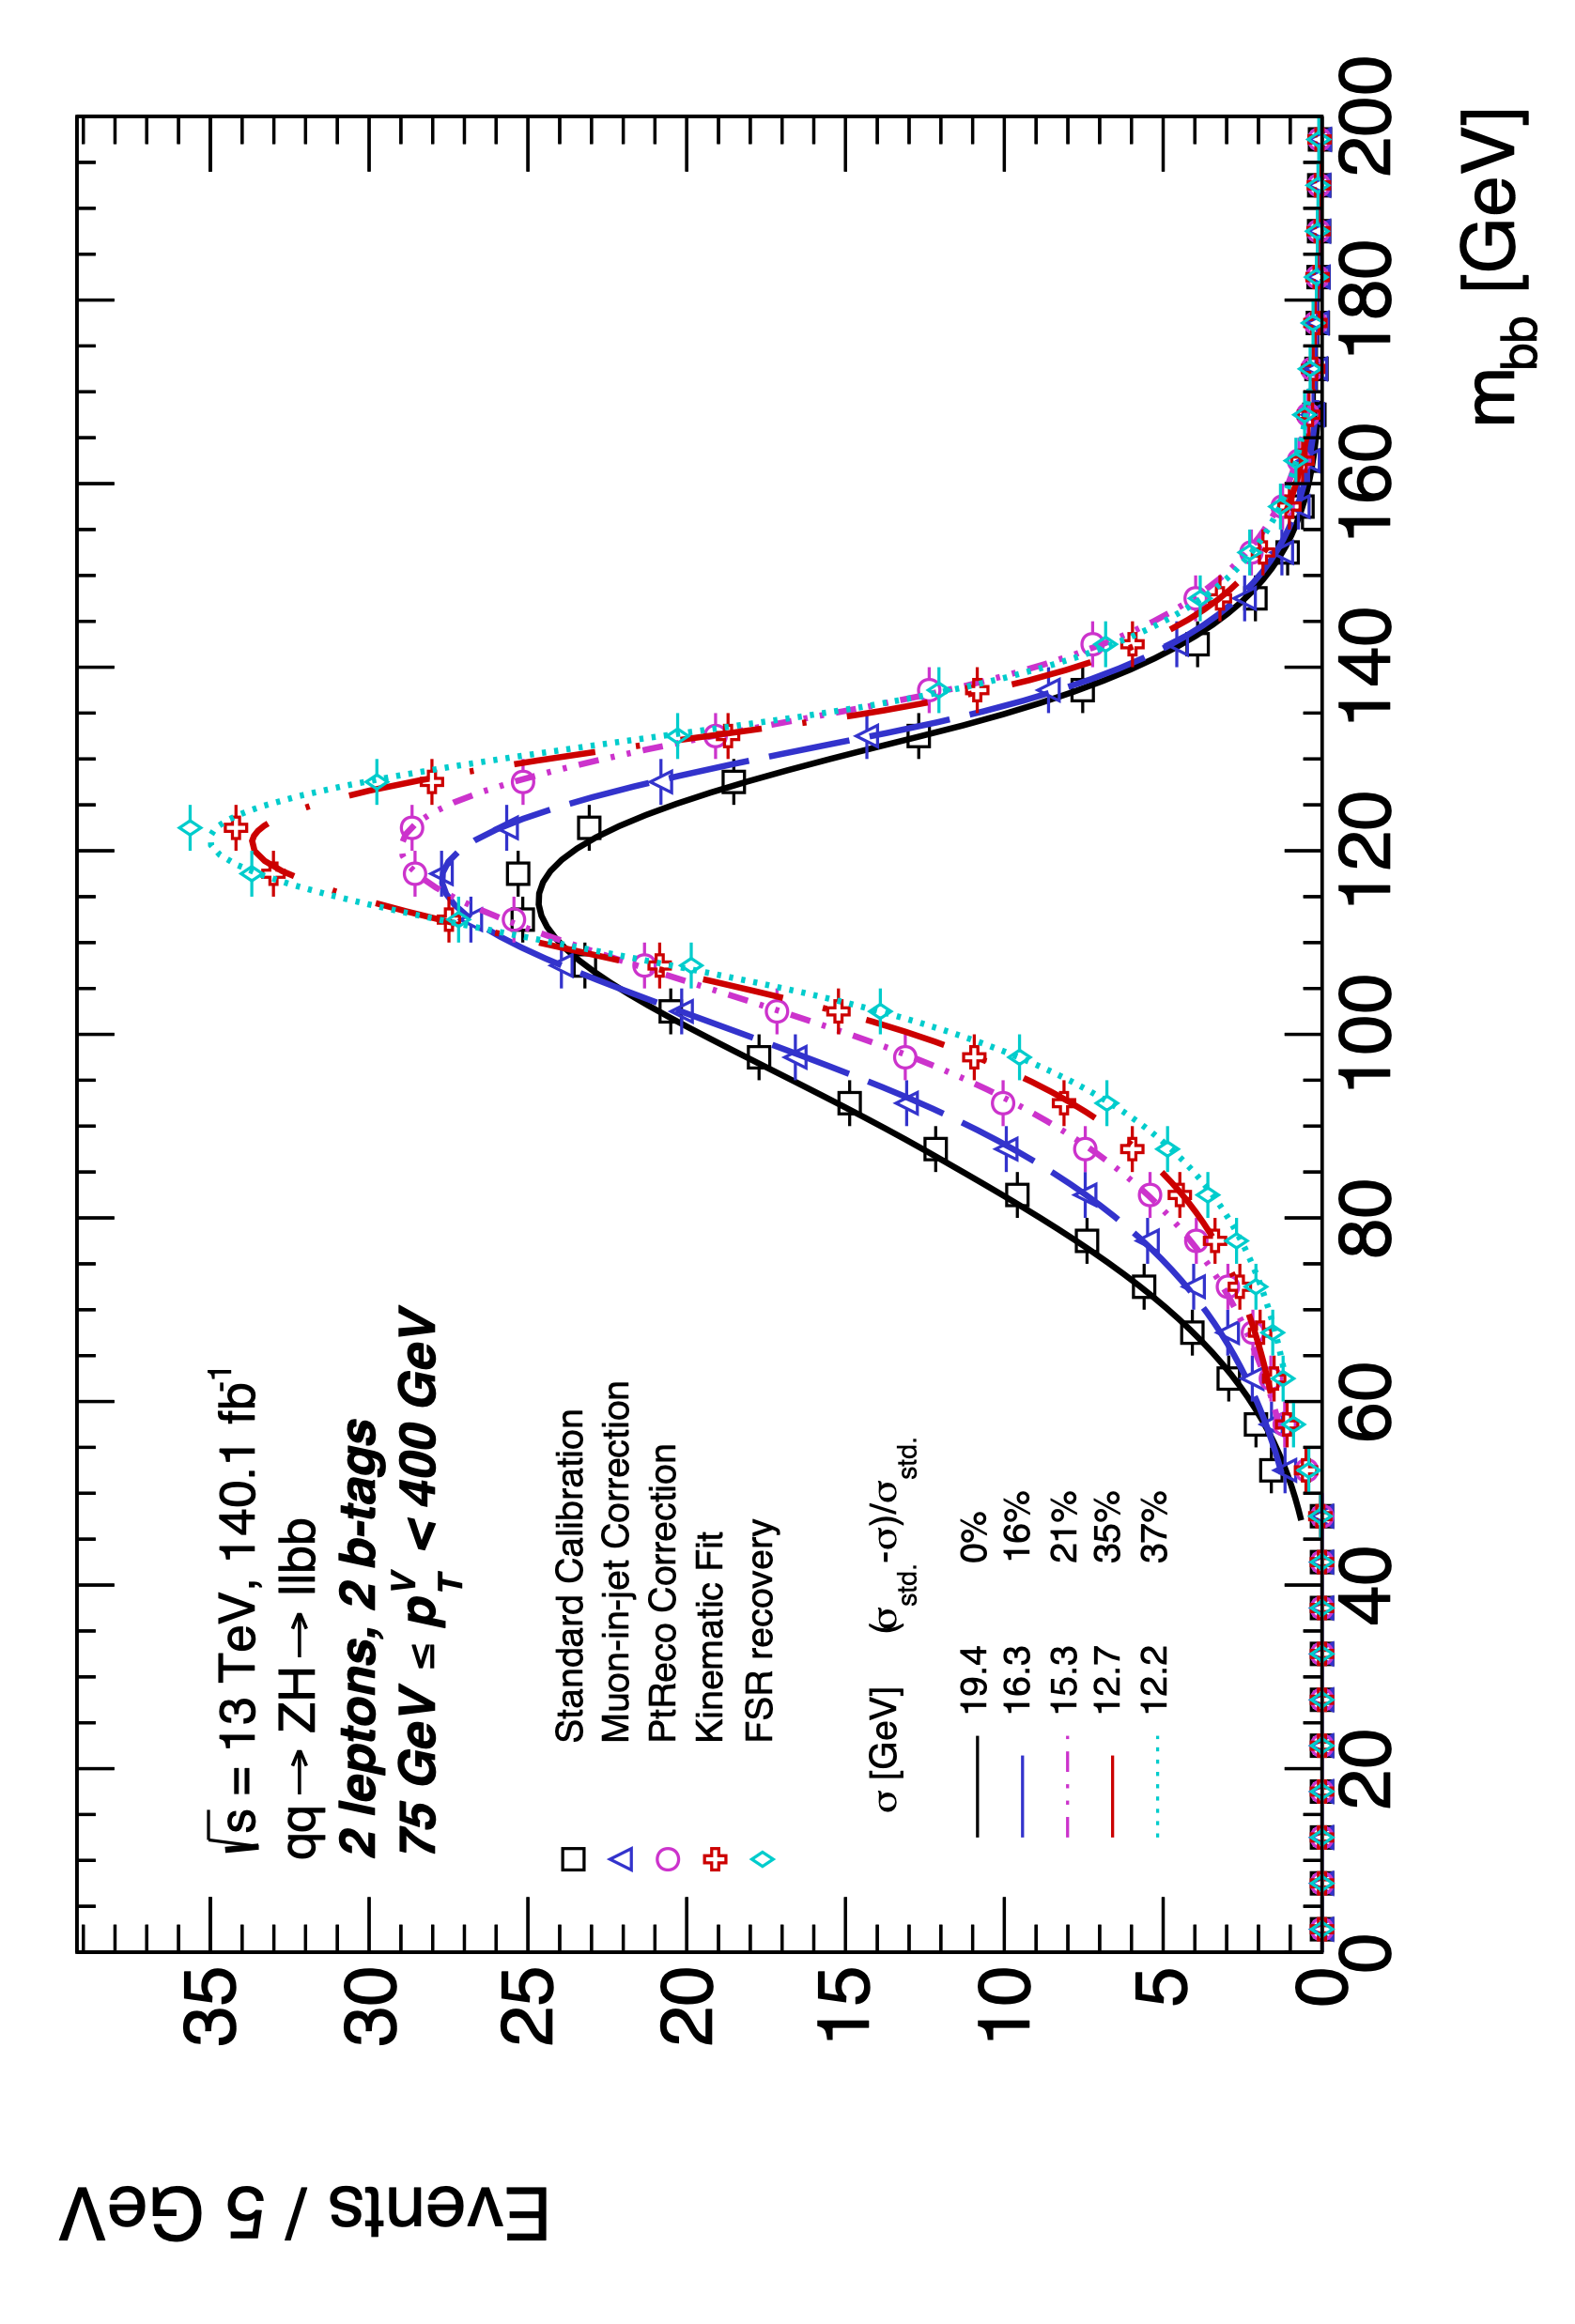
\includegraphics[width=\textwidth]{Images/VH/Correct/CorrectedDist/bbR.png}
  \caption{Resolved \vhb.} 
  \end{subfigure}
  \begin{subfigure}[b]{0.49\textwidth}
    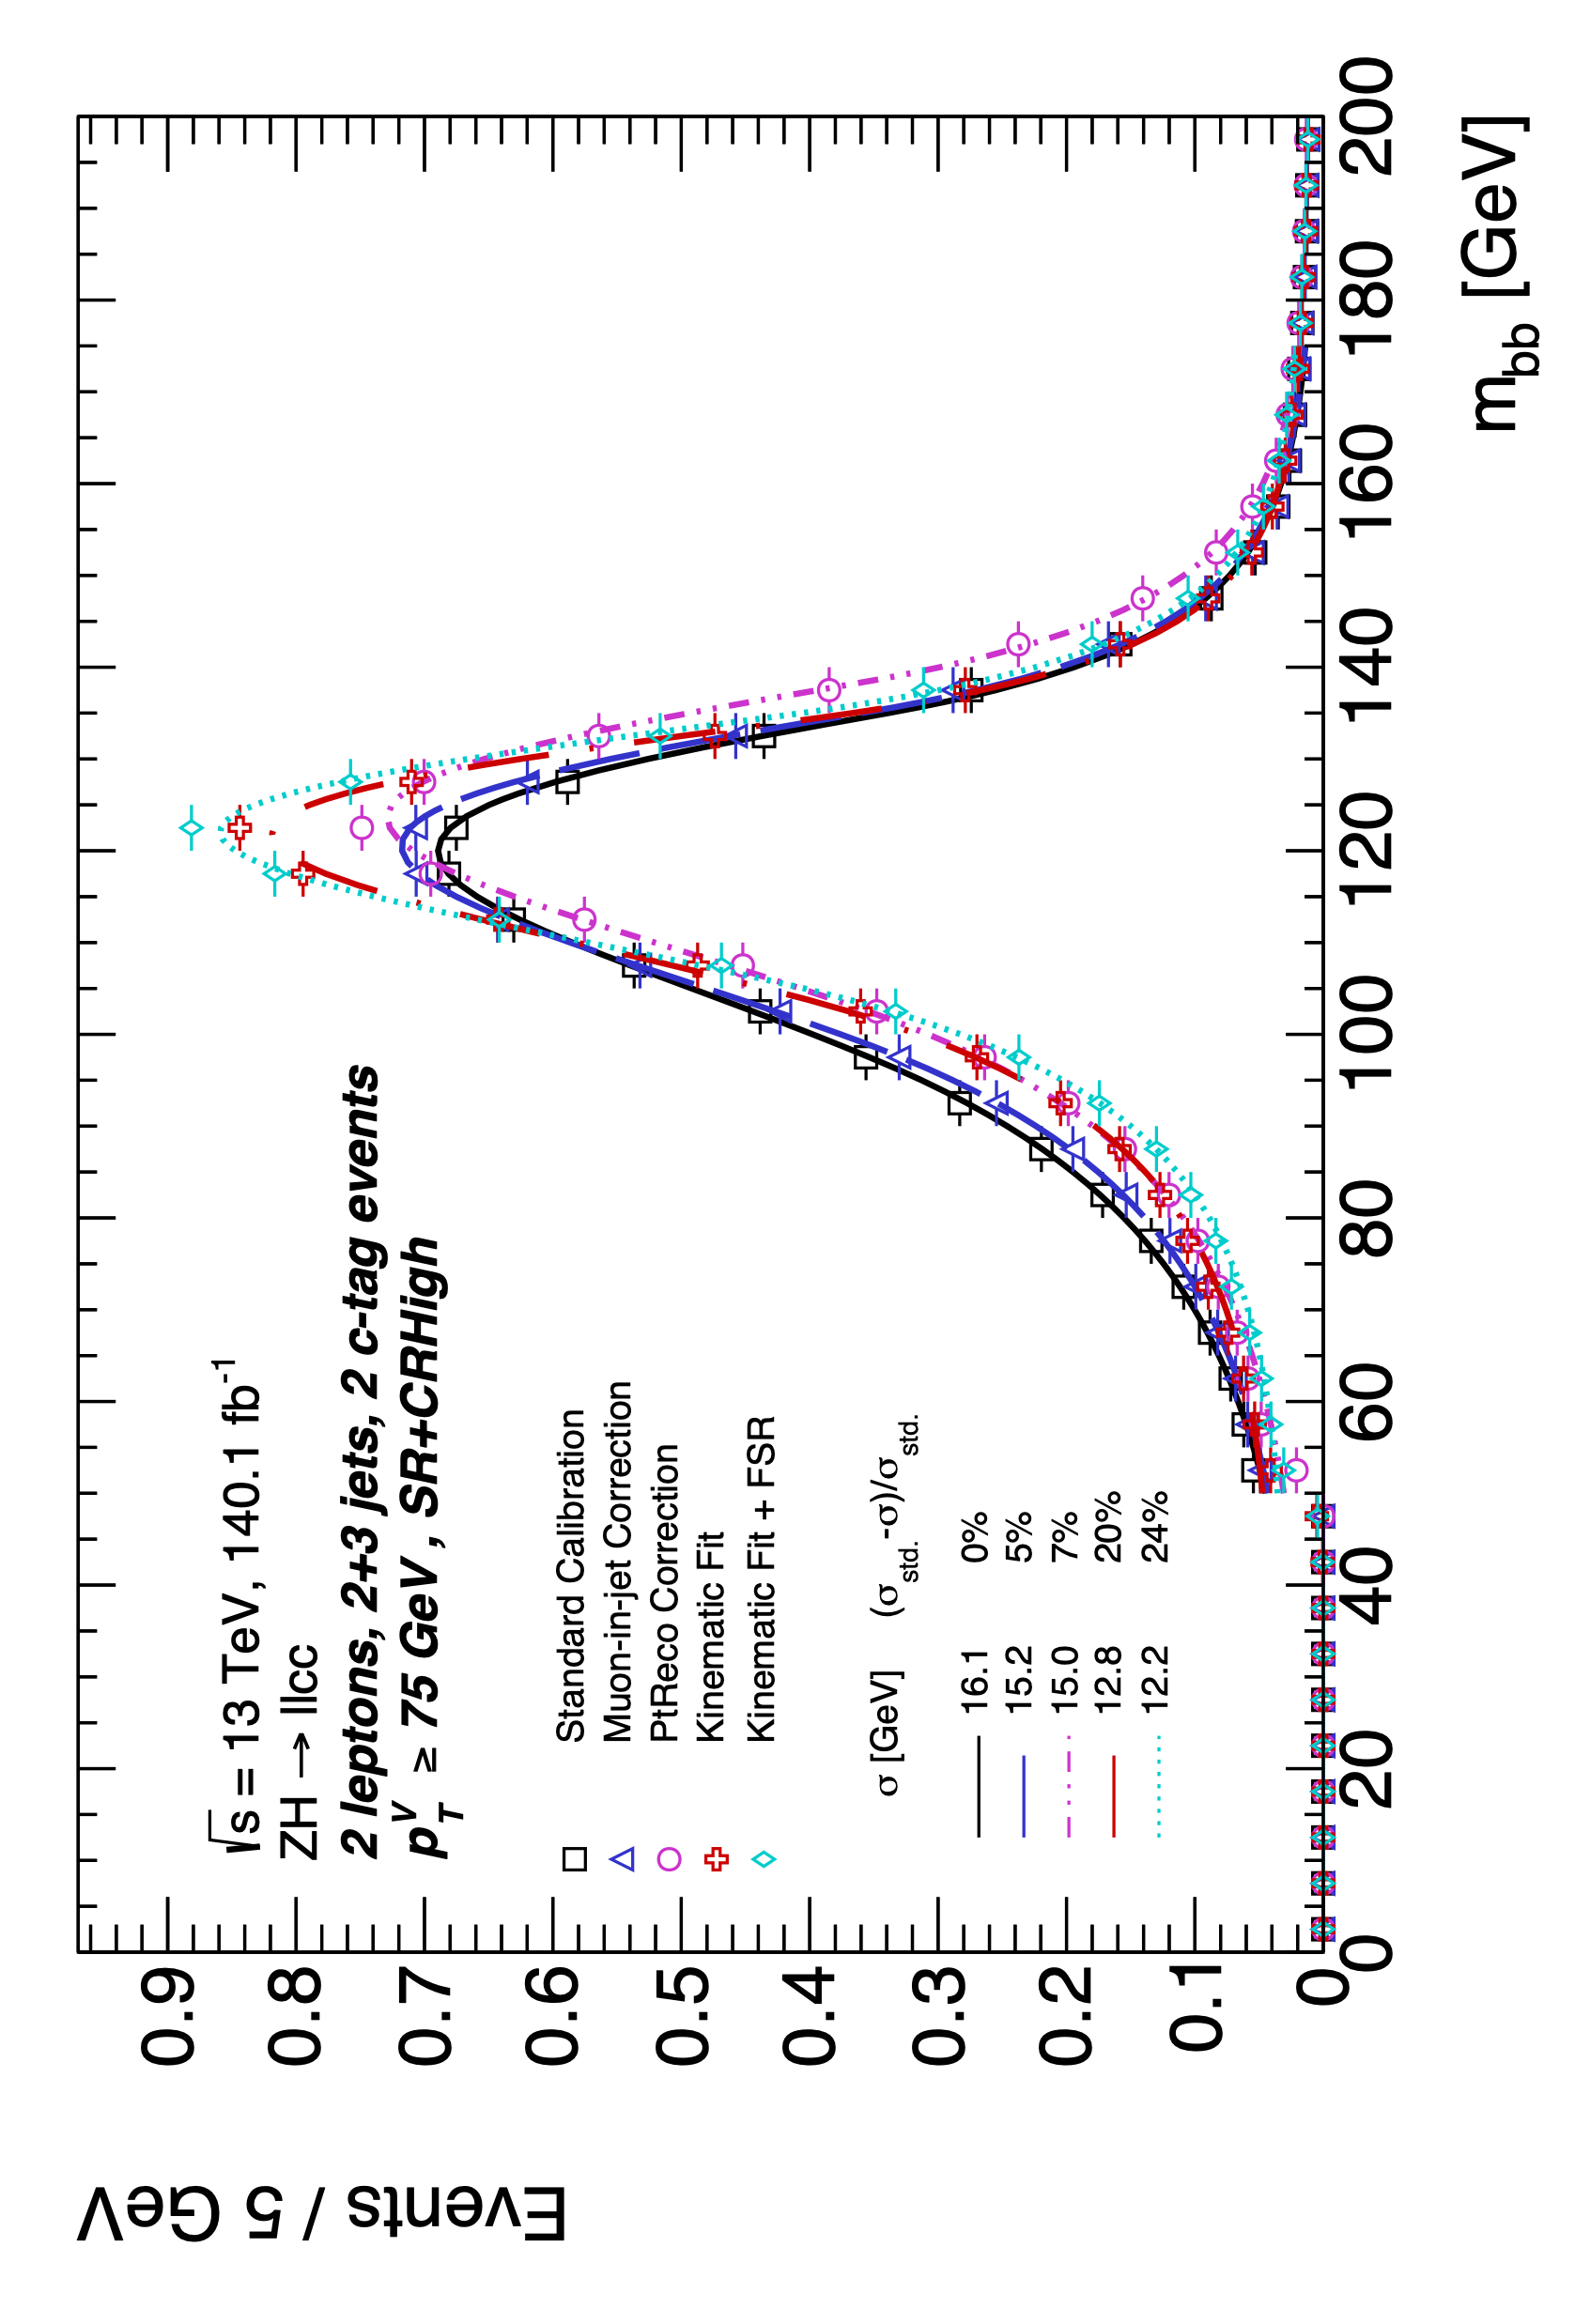
\includegraphics[width=\textwidth]{Images/VH/Correct/CorrectedDist/ccR.png}
    \caption{Resolved \vhc\ with 2 $c$-tags.}
  \end{subfigure} \\
  \begin{subfigure}[b]{0.49\textwidth}
    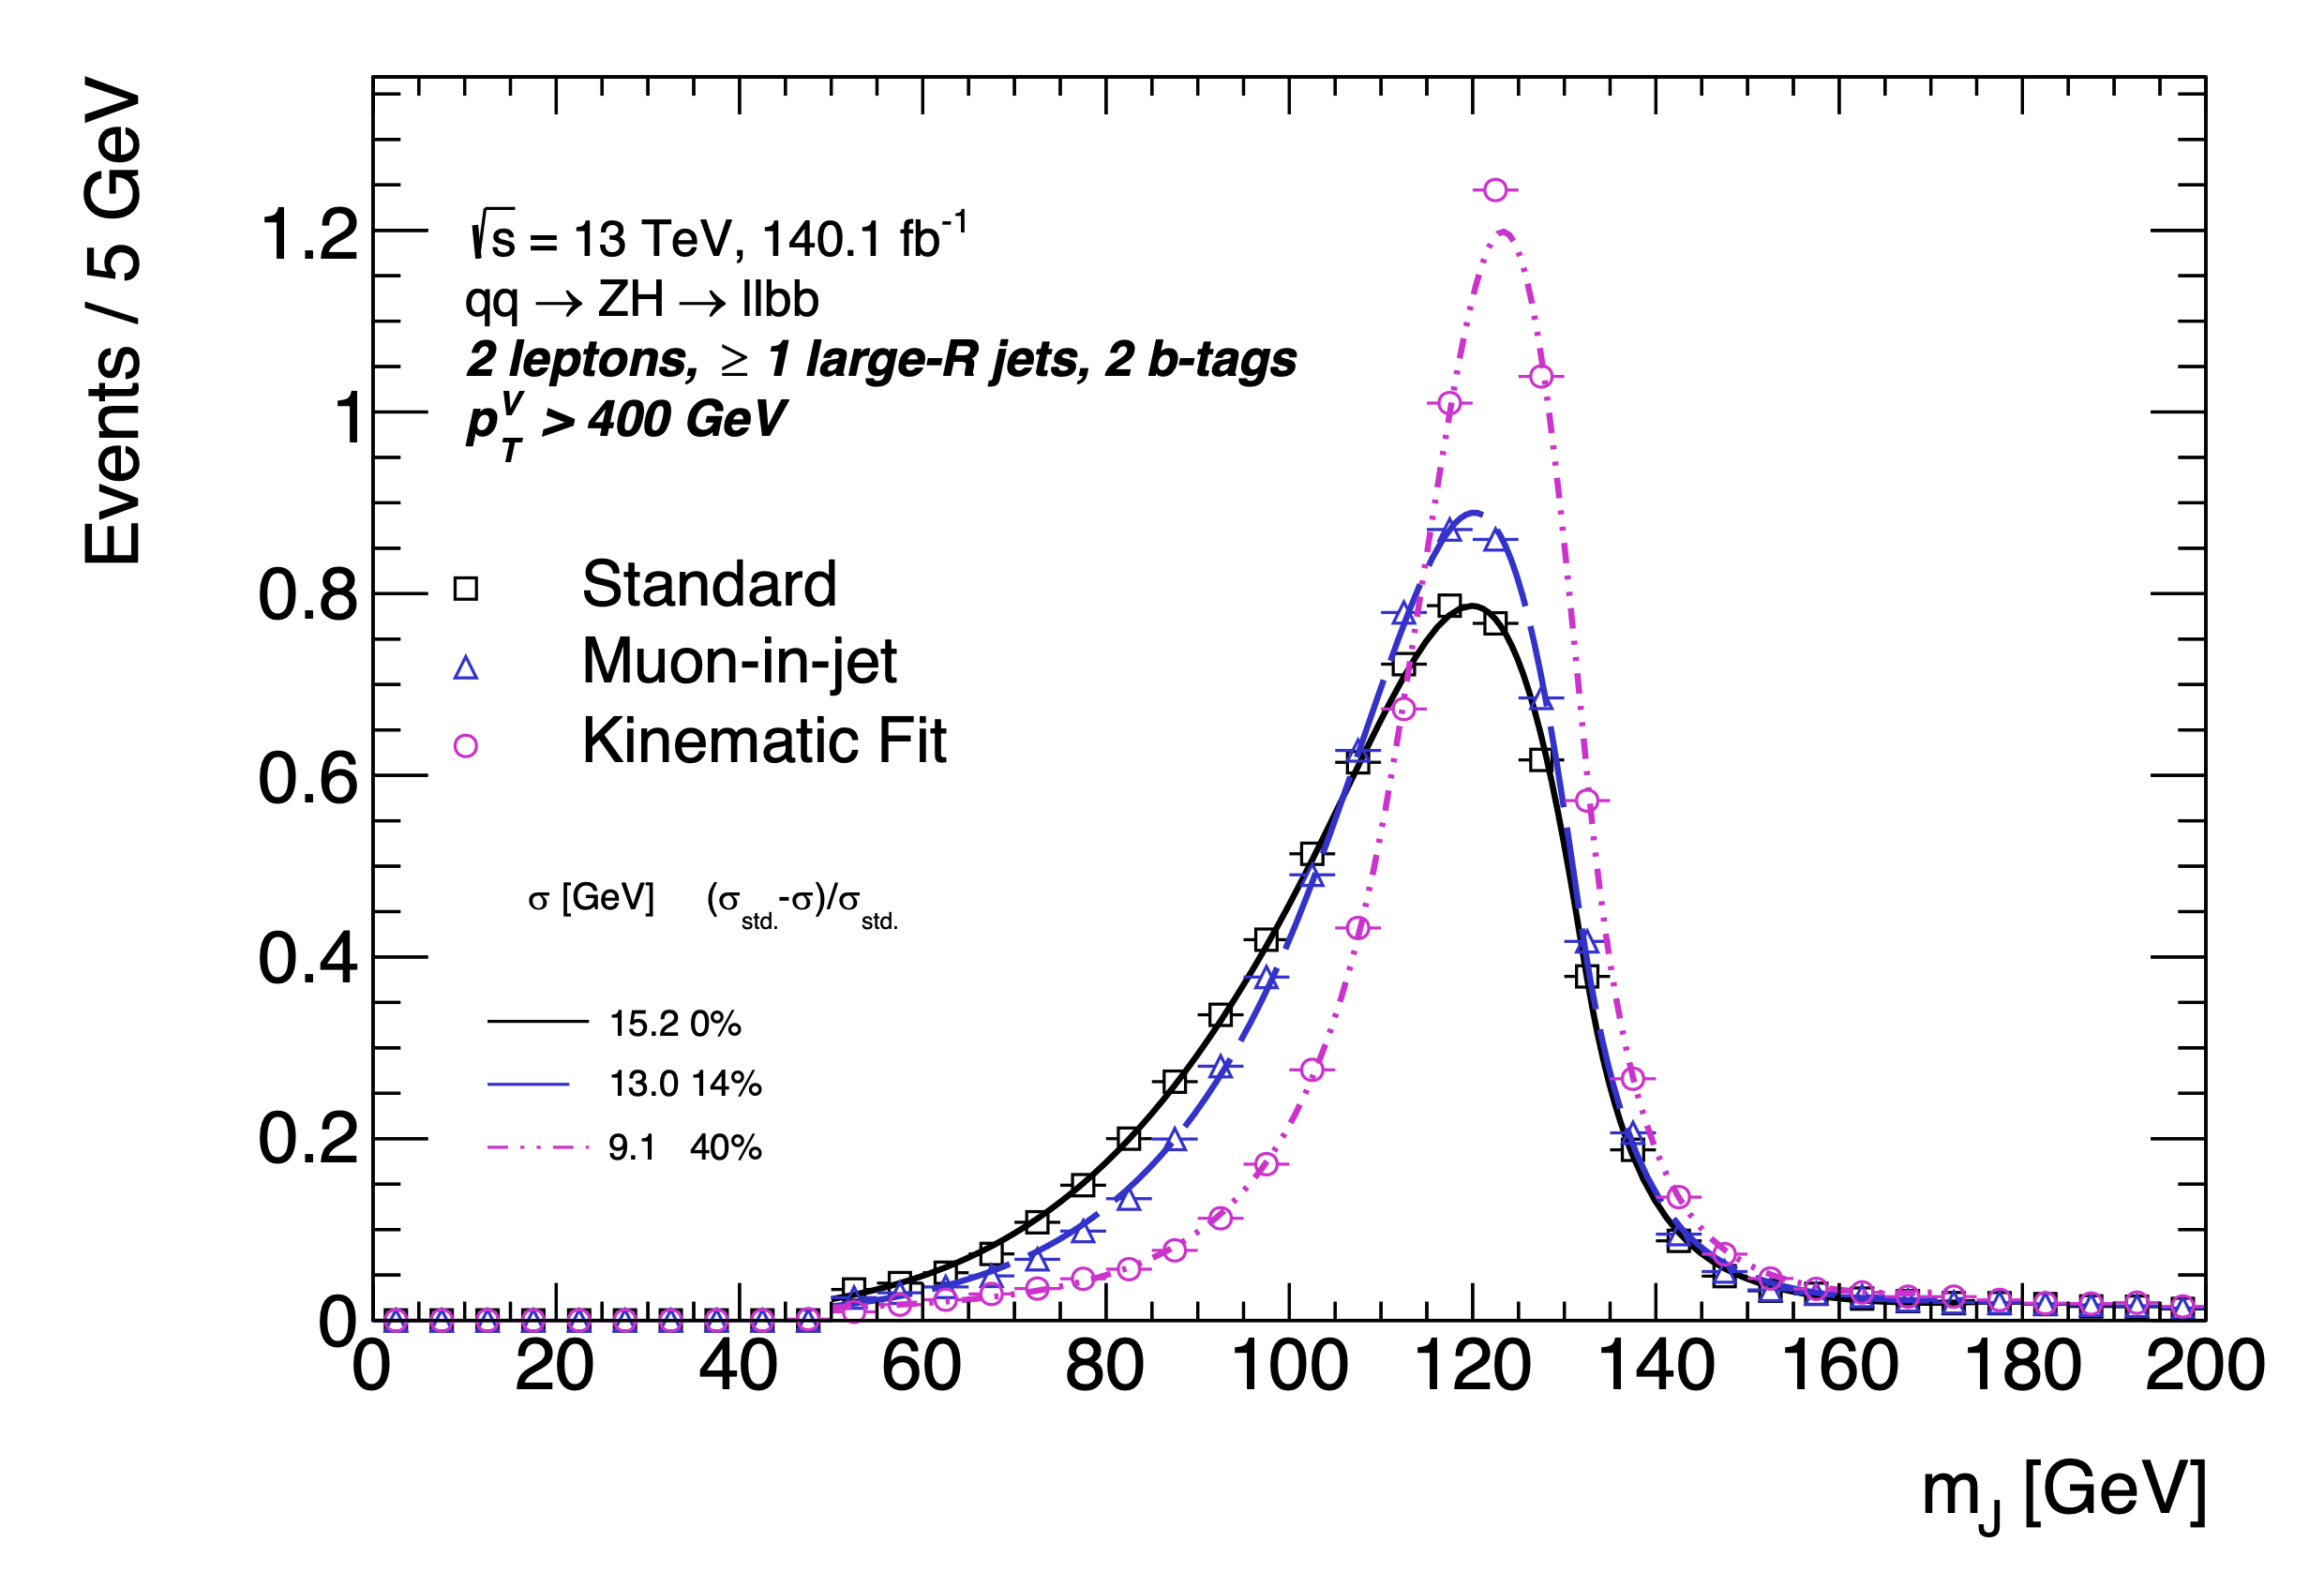
\includegraphics[width=\textwidth]{Images/VH/Correct/CorrectedDist/bbB.png}
    \caption{Boosted \vhb.}
  \end{subfigure}
  \caption{Performance of the energy corrections on simulated samples of different analysis schemes in the 2-lepton channels, inclusive in \ptv\ and number of jets.}
  \label{fig:CorrResults}
\end{figure} 
The effects of the different reconstruction techniques are illustrated in Figure~\ref{fig:CorrResults} for some selected 2-lepton resolved and boosted distributions. 